\documentclass[12pt,a4paper]{article}

% ── Kodowanie i język ──────────────────────────────────────────────────────────
\usepackage[T1]{fontenc}
\usepackage[utf8]{inputenc}
\usepackage[polish]{babel}

% ── Marginesy ─────────────────────────────────────────────────────────────────
\usepackage[top=2.5cm, bottom=2.5cm, left=2.5cm, right=2.5cm]{geometry}

% ── Typografia ────────────────────────────────────────────────────────────────
\usepackage{parskip}
\setlength{\parskip}{6pt}

% ── Kolory i linki ────────────────────────────────────────────────────────────
\usepackage[dvipsnames]{xcolor}
\usepackage{hyperref}
\hypersetup{
	colorlinks=true,
	linkcolor=MidnightBlue,
	urlcolor=MidnightBlue,
	citecolor=MidnightBlue
}

% ── Grafiki ───────────────────────────────────────────────────────────────────
\usepackage{graphicx}
\usepackage{float}
\graphicspath{{./figures/}}

% ── Tabele ────────────────────────────────────────────────────────────────────
\usepackage{booktabs}
\usepackage{tabularx}
\usepackage{array}
\usepackage{multirow}

% ── Kod źródłowy ──────────────────────────────────────────────────────────────
\usepackage{listings}
\lstset{
	basicstyle=\ttfamily\footnotesize,
	backgroundcolor=\color{gray!8},
	frame=single,
	rulecolor=\color{gray!40},
	breaklines=true,
	captionpos=b,
	language=Python,
	showstringspaces=false,
	keywordstyle=\color{MidnightBlue}\bfseries,
	commentstyle=\color{gray},
	stringstyle=\color{OliveGreen},
	numbers=left,
	numberstyle=\tiny\color{gray},
	numbersep=8pt
}

% ── Nagłówki sekcji ───────────────────────────────────────────────────────────
\usepackage{titlesec}
\titleformat{\section}{\large\bfseries}{{\thesection.}}{0.5em}{}[\titlerule]
\titleformat{\subsection}{\normalsize\bfseries}{{\thesubsection}}{0.5em}{}
\titleformat{\subsubsection}{\normalsize\itshape}{{\thesubsubsection}}{0.5em}{}

% ── Pozostałe ─────────────────────────────────────────────────────────────────
\usepackage{amsmath}
\usepackage{enumitem}
\setlist{noitemsep, topsep=4pt}
\usepackage{caption}
\captionsetup{font=small, labelfont=bf}

% ── Nagłówek/stopka ───────────────────────────────────────────────────────────
\usepackage{fancyhdr}
\pagestyle{fancy}
\fancyhf{}
\rhead{\small Predykcja Cen Biletów Lotniczych}
\lhead{\small Eksploracja Danych}
\rfoot{\thepage}
\renewcommand{\headrulewidth}{0.4pt}

% ══════════════════════════════════════════════════════════════════════════════
\begin{document}
	
	% ── Strona tytułowa ───────────────────────────────────────────────────────────
	\begin{titlepage}
		\centering
		\vspace*{2cm}
		{\LARGE\bfseries Predykcja Cen Biletów Lotniczych\\[0.4em]
			Analiza i Modelowanie\par}
		\vspace{1.5cm}
		{\large Projekt z przedmiotu: \textbf{Eksploracja Danych}\par}
		\vspace{0.8cm}
		\rule{0.6\textwidth}{0.4pt}\\[0.8cm]
		{\normalsize Autor: Jakub Szamik\par}
		\vspace{0.4cm}
		{\normalsize 2025\par}
		\vfill
		{\small Zbiór danych: \textit{Flight Price Prediction} (Kaggle)\\
			\url{https://www.kaggle.com/datasets/shubhambathwal/flight-price-prediction}\par}
		\vspace{1cm}
	\end{titlepage}
	
	\thispagestyle{empty}
	\tableofcontents
	\newpage
	
	% ══════════════════════════════════════════════════════════════════════════════
	\section*{Streszczenie}
	\addcontentsline{toc}{section}{Streszczenie}
	
	Projekt dotyczy predykcji cen biletów lotniczych na podstawie zbioru
	\textit{Flight Price Prediction} (Kaggle) zawierającego ponad 300\,000 rekordów
	z tras krajowych w Indiach. Cel: zbudowanie modelu regresyjnego o możliwie
	najwyższej dokładności predykcji ceny biletu (w INR).
	
	Zastosowano podejście wieloetapowe: eksploracja danych (EDA), wykrywanie anomalii
	metodą \textbf{Isolation Forest}, porównanie sześciu algorytmów uczenia maszynowego
	(LinearRegression, Ridge, Random Forest, Gradient Boosting, XGBoost, LightGBM),
	ewaluacja z krzyżową walidacją i tuningiem hiperparametrów. Jako modele finalne
	wybrano \textbf{LightGBM} --- osobno dla klasy Economy i Business. Wyjaśnialność
	decyzji modeli przeanalizowano metodą \textbf{SHAP}.
	
	
	% ══════════════════════════════════════════════════════════════════════════════
	\section{Wybór Zbioru Danych}
	
	Analizowany zbiór danych pochodzi z portalu Kaggle i nosi nazwę
	\textit{Flight Price Prediction} (\texttt{Clean\_Dataset.csv}).
	Zawiera informacje o cenach biletów lotniczych na trasach krajowych w Indiach,
	zebrane dla sześciu głównych linii lotniczych obsługujących sześć miast.
	Zbiór liczy \textbf{ponad 300\,000 rekordów} i jest gotowy do użycia ---
	nie zawiera brakujących wartości.
	
	Zbiór wyróżnia się ze względu na:
	\begin{itemize}
		\item dużą liczebność umożliwiającą wiarygodną ewaluację modeli,
		\item naturalny podział na dwa segmenty cenowe (Economy / Business),
		\item obecność silnych zależności nieliniowych (efekt \textit{last-minute}),
		\item dostępność zarówno zmiennych numerycznych, jak i kategorycznych.
	\end{itemize}
	
	\noindent\textbf{Źródło:}
	\url{https://www.kaggle.com/datasets/shubhambathwal/flight-price-prediction}
	
	% ══════════════════════════════════════════════════════════════════════════════
	\section{Definicja Problemu i Charakterystyka Zbioru}
	
	\subsection{Problem predykcyjny}
	
	Celem jest zbudowanie modelu \textbf{regresji nadzorowanej} prognozującego cenę
	biletu lotniczego (zmienna \texttt{price}, w INR) na podstawie dostępnych cech
	opisujących rejs. Zmienna docelowa jest ciągła --- zadanie klasyfikowane jako
	regresja.
	
	\subsection{Zmienne w zbiorze}
	
	\begin{table}[H]
		\centering
		\begin{tabularx}{\textwidth}{llXl}
			\toprule
			\textbf{Zmienna} & \textbf{Kodowanie} & \textbf{Opis} & \textbf{Typ} \\
			\midrule
			\texttt{airline}           & One-Hot & Linia lotnicza (6 kategorii)           & kategoryczna \\
			\texttt{source\_city}      & One-Hot & Miasto wylotu (6 miast)                & kategoryczna \\
			\texttt{destination\_city} & One-Hot & Miasto przylotu (6 miast)              & kategoryczna \\
			\texttt{departure\_time}   & One-Hot & Pora dnia odlotu (6 pasm)              & kategoryczna \\
			\texttt{arrival\_time}     & One-Hot & Pora dnia przylotu (6 pasm)            & kategoryczna \\
			\texttt{stops}             & numerycznie & Liczba przesiadek: 0, 1, 2+        & porządkowa   \\
			\texttt{duration}          & ---     & Czas trwania lotu (godz.)              & numeryczna   \\
			\texttt{days\_left}        & ---     & Liczba dni do wylotu                   & numeryczna   \\
			\texttt{class}             & 0/1     & Klasa podróży (Economy=0, Business=1)  & binarna      \\
			\texttt{price}             & ---     & \textbf{Cena biletu w INR (cel)}       & numeryczna   \\
			\bottomrule
		\end{tabularx}
		\caption{Zmienne w zbiorze danych wraz ze strategią kodowania}
	\end{table}
	
	\subsection{Podstawowe statystyki}
	
	Zmienna docelowa \texttt{price} charakteryzuje się znaczną asymetrią prawostronną
	--- mediana wyraźnie odbiega od średniej, co sugeruje obecność obserwacji
	odstających po prawej stronie rozkładu. Ceny biletów klasy Business są
	wielokrotnie wyższe niż Economy, co uzasadnia późniejsze modelowanie osobne dla
	każdej klasy.
	
	% ══════════════════════════════════════════════════════════════════════════════
	\section{Przegląd Literatury}
	
	Predykcja cen biletów lotniczych jest aktywnie badanym problemem w literaturze
	uczenia maszynowego. Poniżej zebrano kluczowe prace stanowiące punkt odniesienia
	dla niniejszej analizy.
	
	\begin{itemize}
		\item \textbf{Groves \& Gini (2011)} --- jedno z pierwszych zastosowań ML
		(regresja liniowa, SVM) do prognozowania cen lotów. Autorzy wskazują na silną
		nieliniowość zależności cena--czas do wylotu.
		
		\item \textbf{Janssen et al. (2015)} --- analiza dynamicznego ustalania cen
		(\textit{dynamic pricing}) linii lotniczych; potwierdzono, że ceny rosną
		wykładniczo w ostatnich tygodniach przed wylotem.
		
		\item \textbf{Tziridis et al. (2017)} --- porównanie modeli (regresja liniowa,
		Random Forest, sieci neuronowe) na danych greckich linii lotniczych; Random
		Forest uzyskał najniższy MAE.
		
		\item \textbf{Liu et al. (2008) --- Isolation Forest} --- metoda detekcji
		anomalii zastosowana w niniejszym projekcie. Algorytm izoluje obserwacje
		odstające przez losowe partycjonowanie przestrzeni cech.
		
		\item \textbf{Chen \& Guestrin (2016) --- XGBoost} oraz
		\textbf{Ke et al. (2017) --- LightGBM} --- wiodące algorytmy gradientowego
		boostingu osiągające wysokie wyniki w zadaniach regresji na danych tabelarycznych.
		
		\item \textbf{Lundberg \& Lee (2017) --- SHAP} --- metoda wyjaśnialności modeli
		ML oparta na teorii gier Shapleya, zastosowana w sekcji~\ref{sec:xai} do
		interpretacji decyzji modeli drzewiastych.
	\end{itemize}
	
	\noindent\textbf{Wnioski z literatury:} modele zespołowe (Random Forest, XGBoost,
	LightGBM) konsekwentnie przewyższają modele liniowe w zadaniach regresji cen
	lotniczych. Kluczowymi predyktorami są: \texttt{days\_left}, \texttt{duration}
	oraz klasa podróży.
	
	% ══════════════════════════════════════════════════════════════════════════════
	\section{Czyszczenie Danych i Selekcja Cech}
	
	\subsection{Wstępna obróbka i kodowanie}
	
	Dane wczytano bez konieczności obsługi brakujących wartości (\texttt{isnull().any()} zwraca \texttt{False}). Wykonano następujące przekształcenia wstępne:
	
	\begin{itemize}
		\item usunięto kolumnę \texttt{Unnamed: 0} (indeks artefaktowy z CSV),
		\item \texttt{stops}: zmapowano \texttt{zero}$\to$0, \texttt{one}$\to$1,
		\texttt{two\_or\_more}$\to$2,
		\item \texttt{class}: zmapowano \texttt{Economy}$\to$0, \texttt{Business}$\to$1
		(kolumna \texttt{is\_business}),
		\item \texttt{departure\_time}: zmapowano na skalę porządkową 1--6
		(Early Morning$\to$1, \ldots, Late Night$\to$6).
	\end{itemize}
	
	\subsection{Usunięcie wartości ekstremalnych}
	
	Na podstawie rozkładu zmiennej \texttt{price} usunięto obserwacje z ceną powyżej
	\textbf{75\,000 INR} jako wartości skrajne niereprezentatywne dla typowego rynku.
	Odsetek usuniętych rekordów wyniósł poniżej 1\% całego zbioru. Wynik
	oczyszczony zapisano jako \texttt{df\_clean}.
	
	\subsection{Wykrywanie anomalii --- Isolation Forest}
	
	Metoda Isolation Forest (Liu et al., 2008) identyfikuje anomalie przez losowe
	partycjonowanie przestrzeni cech i pomiar liczby podziałów potrzebnych do
	izolacji obserwacji. Obserwacje wymagające mniejszej liczby podziałów uznawane
	są za anomalie.
	
	Przetestowano dwa poziomy parametru \texttt{contamination}: \textbf{0,01}
	(1\% odrzuconych) oraz \textbf{0,05} (5\% odrzuconych). Do detekcji użyto
	zmiennych: \texttt{price}, \texttt{duration}, \texttt{days\_left}.
	
	\begin{figure}[H]
		\centering
		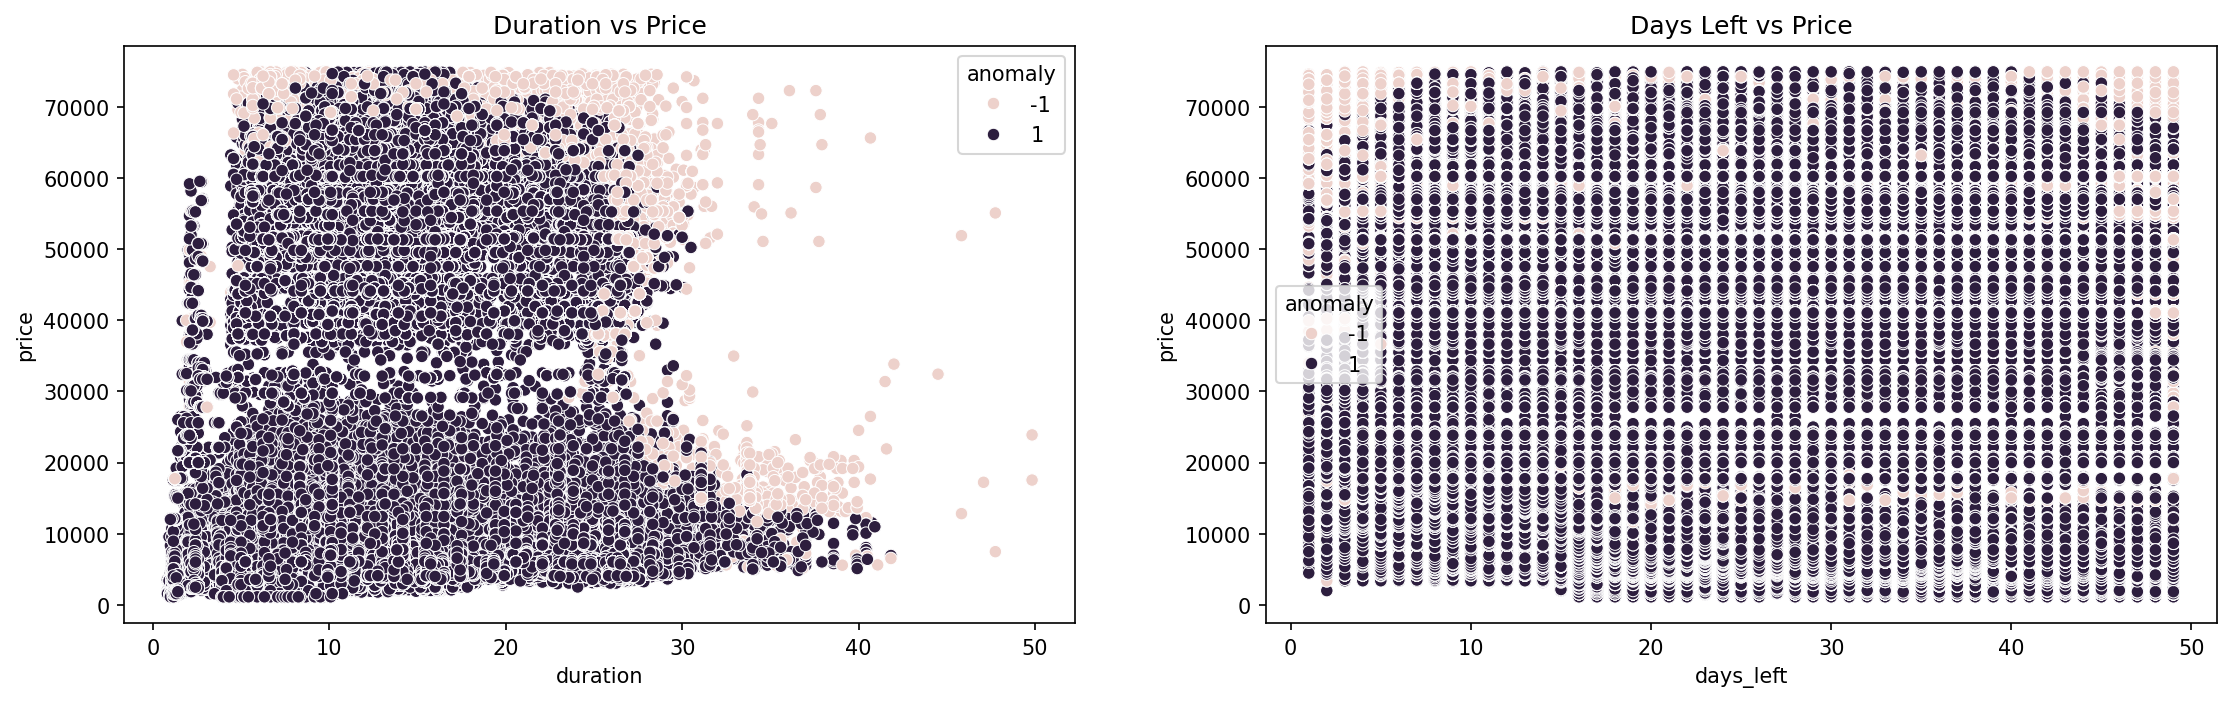
\includegraphics[width=0.93\textwidth]{isolation_forest.png}
		\caption{Detekcja anomalii metodą Isolation Forest (contamination = 0,01 i 0,05)}
	\end{figure}
	
	\subsection{Warianty zbioru danych}
	
	Na potrzeby porównania wpływu usunięcia anomalii wydzielono trzy wersje:
	
	\begin{table}[H]
		\centering
		\begin{tabularx}{0.8\textwidth}{lXl}
			\toprule
			\textbf{Zbiór} & \textbf{Opis} & \textbf{Contamination} \\
			\midrule
			\texttt{df1} & Pełny \texttt{df\_clean}, anomalie nieusunięte & --- \\
			\texttt{df2} & Anomalie usunięte (1\% obserwacji odrzuconych) & 0,01 \\
			\texttt{df3} & Anomalie usunięte (5\% obserwacji odrzuconych) & 0,05 \\
			\bottomrule
		\end{tabularx}
		\caption{Trzy warianty zbioru danych}
	\end{table}
	
	\subsection{Wstępna selekcja cech}
	
	Usunięto kolumnę \texttt{flight} (identyfikator lotu bez wartości predykcyjnej).
	Zmienne kategoryczne (\texttt{airline}, \texttt{source\_city},
	\texttt{destination\_city}, \texttt{departure\_time}, \texttt{arrival\_time})
	zakodowano metodą \textbf{One-Hot Encoding} z parametrem \texttt{drop\_first=True}
	w celu uniknięcia wieloliniowości.
	
	% ══════════════════════════════════════════════════════════════════════════════
	\section{Eksploracja Danych (EDA)}
	
	\subsection{Rozkład zmiennej docelowej}
	
	Rozkład ceny biletu po odcięciu obserwacji powyżej 75\,000 INR wykazuje wyraźną
	prawostronność --- większość biletów koncentruje się w niskim przedziale
	cenowym, przy nielicznych obserwacjach o wysokich wartościach. Widoczny jest
	bimodalny charakter rozkładu wynikający z podziału na klasę Economy i Business.
	
	\begin{figure}[H]
		\centering
		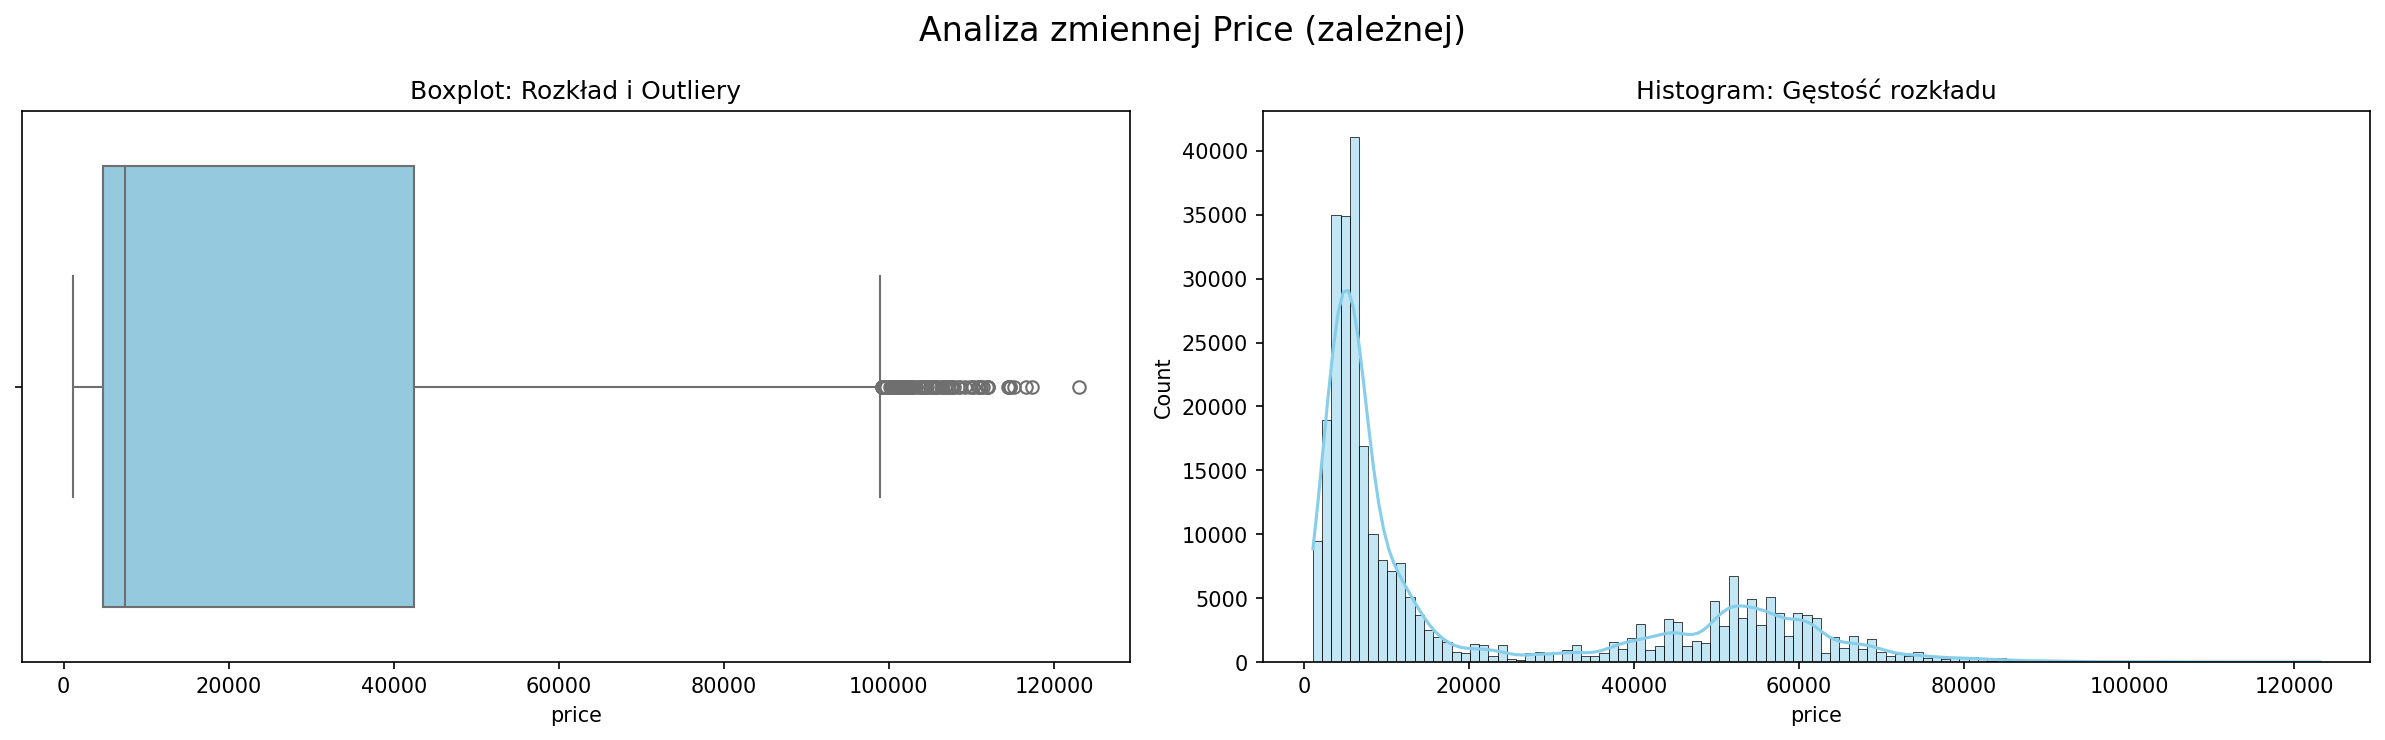
\includegraphics[width=0.93\textwidth]{price_distribution.png}
		\caption{Rozkład zmiennej docelowej \texttt{price} --- boxplot i histogram z KDE}
	\end{figure}
	
	\subsection{Macierz korelacji}
	
	Macierz korelacji Pearsona dla zmiennych numerycznych wskazuje na:
	\begin{itemize}
		\item \textbf{silną korelację} \texttt{is\_business} z \texttt{price} ---
		odzwierciedla fundamentalną różnicę cenową między klasami,
		\item umiarkowaną korelację \texttt{duration} z \texttt{price} ---
		dłuższe trasy są droższe,
		\item słabą, ale widoczną korelację \texttt{days\_left} z \texttt{price} ---
		ceny rosną wraz ze zbliżaniem się terminu wylotu.
	\end{itemize}
	
	\begin{figure}[H]
		\centering
		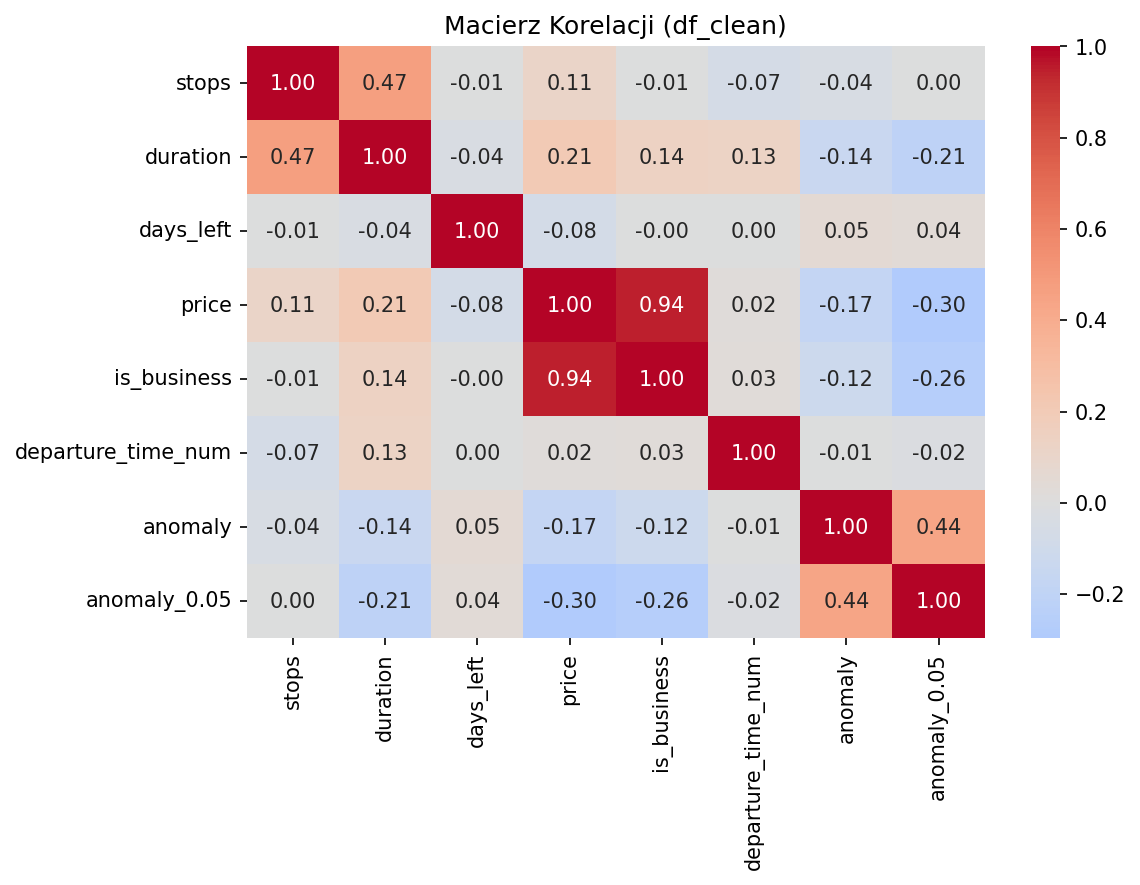
\includegraphics[width=0.93\textwidth]{correlation_matrix.png}
		\caption{Macierz korelacji Pearsona dla zmiennych numerycznych (df\_clean)}
	\end{figure}
	
	\subsection{Rozkład zmiennych kategorycznych}
	
	Analiza rozkładu zmiennych kategorycznych (linia lotnicza, miasto wylotu/przylotu,
	pora odlotu) z obliczeniem współczynnika zmienności CV. Wartość CV $<$ 0,3
	wskazuje na względnie równomierny rozkład --- dane są dobrze zbalansowane
	dla większości zmiennych kategorycznych.
	
	\begin{figure}[H]
		\centering
		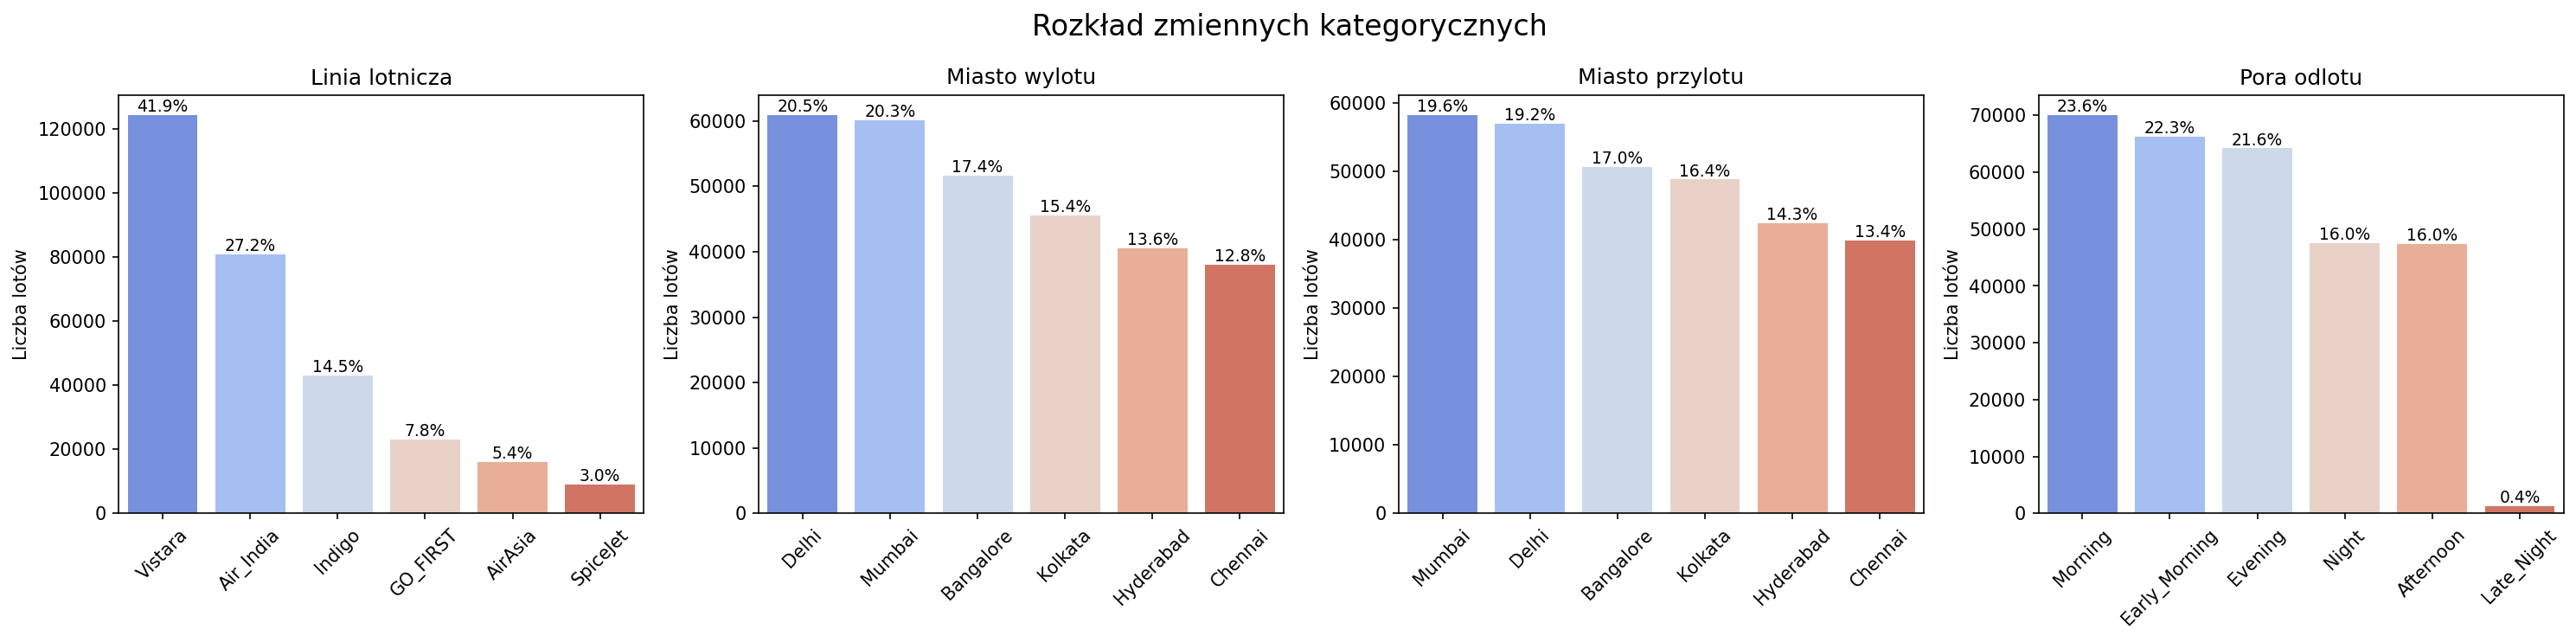
\includegraphics[width=0.93\textwidth]{categorical_distributions.png}
		\caption{Rozkład obserwacji według linii lotniczej, miast i pory odlotu}
	\end{figure}
	
	\subsection{Analiza linii lotniczych i klas podróży}
	
	Zestawienie liczby lotów z podziałem na klasę Economy/Business oraz rozkłady
	cen dla poszczególnych linii. Widoczne jest silne zróżnicowanie cenowe między
	przewoźnikami oraz dominacja biletów klasy Economy w zbiorze.
	
	\begin{figure}[H]
		\centering
		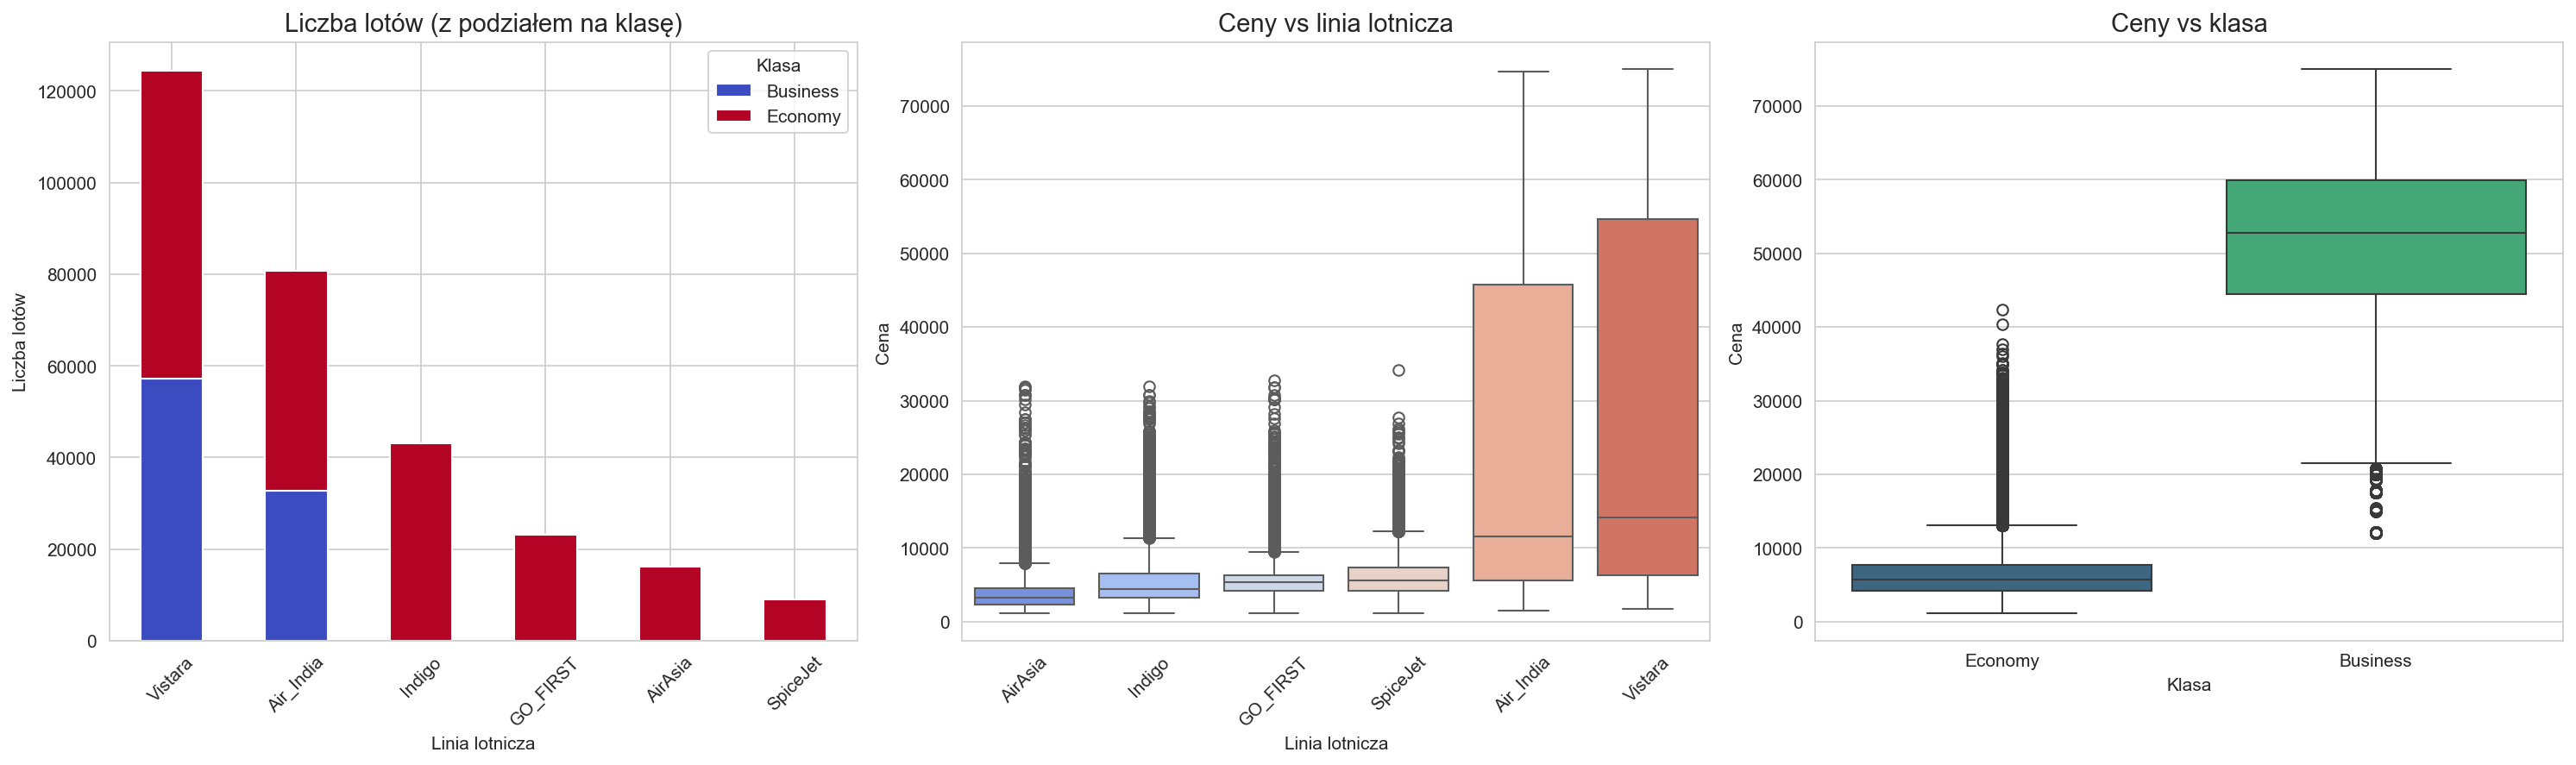
\includegraphics[width=0.93\textwidth]{airline_price_analysis.png}
		\caption{Liczba lotów i rozkład cen według linii lotniczej i klasy podróży}
	\end{figure}
	
	\subsection{Zależność ceny od czasu do wylotu i czasu lotu}
	
	Analiza dotyczy wyłącznie lotów bez przesiadek (\texttt{stops=0}), aby
	wyeliminować wpływ zmiennej \texttt{stops} na czas trwania. Wykresy rozrzutu
	z nałożoną linią trendu (średnia grupowa) potwierdzają nieliniową zależność
	ceny od \texttt{days\_left} --- ceny rosną wykładniczo wraz ze zbliżaniem się
	terminu wylotu, co jest zgodne z modelem \textit{dynamic pricing}
	(Janssen et al., 2015).
	
	\begin{figure}[H]
		\centering
		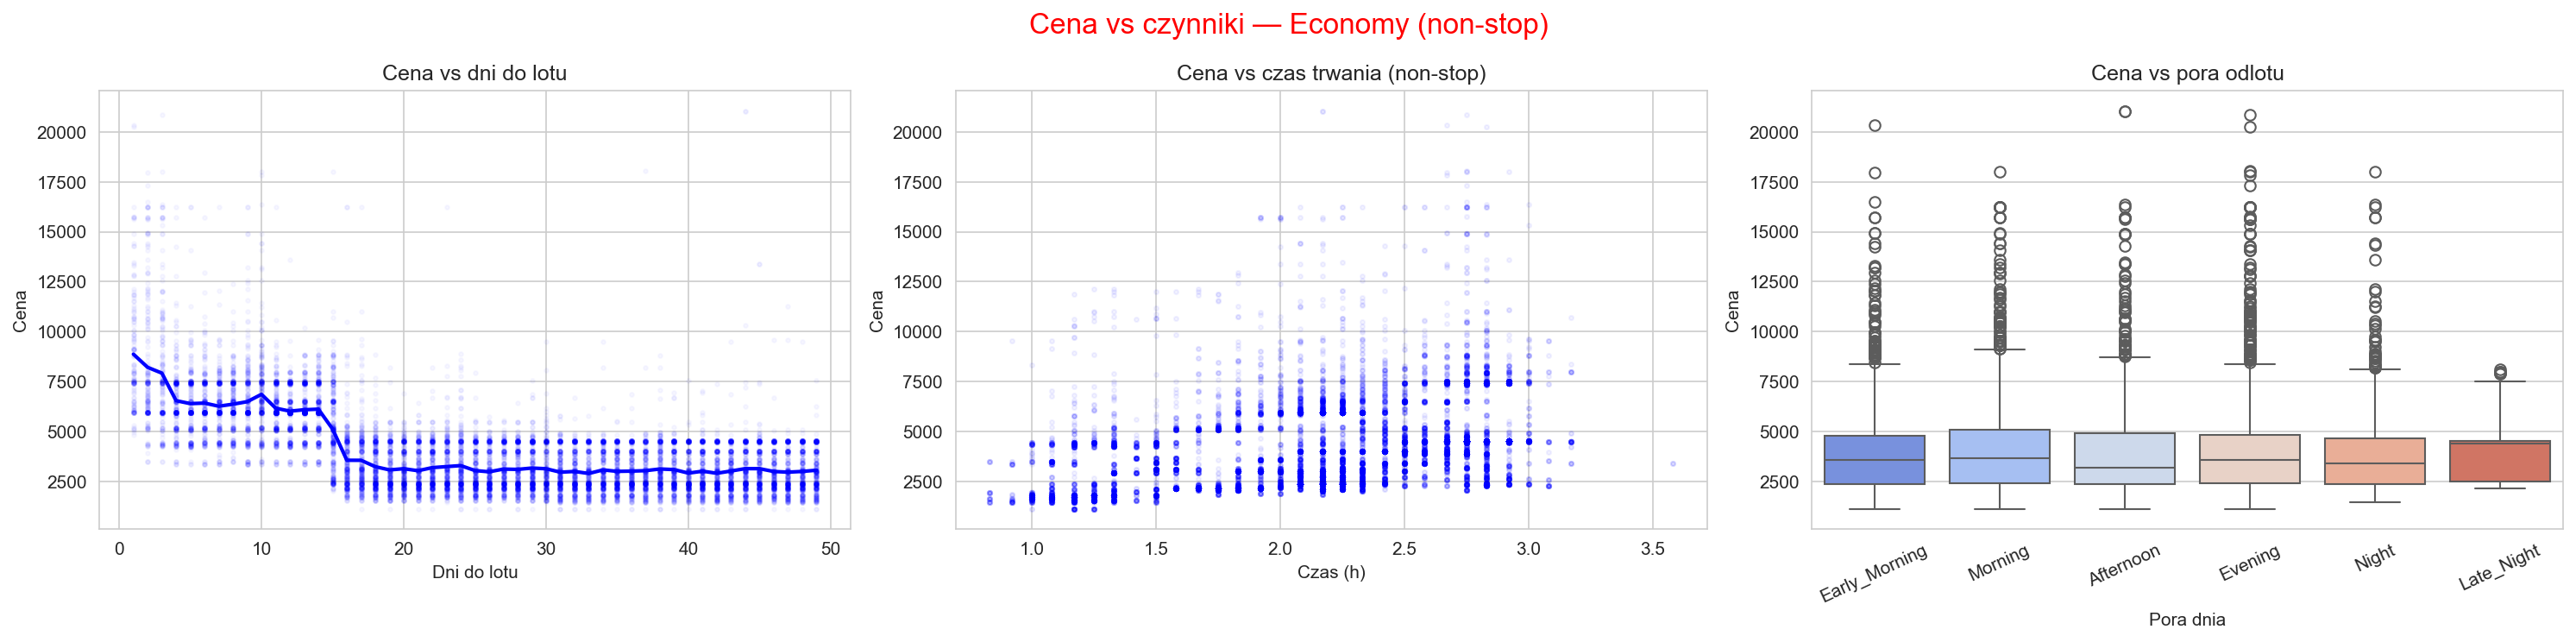
\includegraphics[width=0.93\textwidth]{price_vs_days_duration_economy.png}
		\caption{Zależność ceny od \texttt{days\_left}, \texttt{duration} i pory odlotu --- Economy (loty non-stop)}
	\end{figure}
	
	\begin{figure}[H]
		\centering
		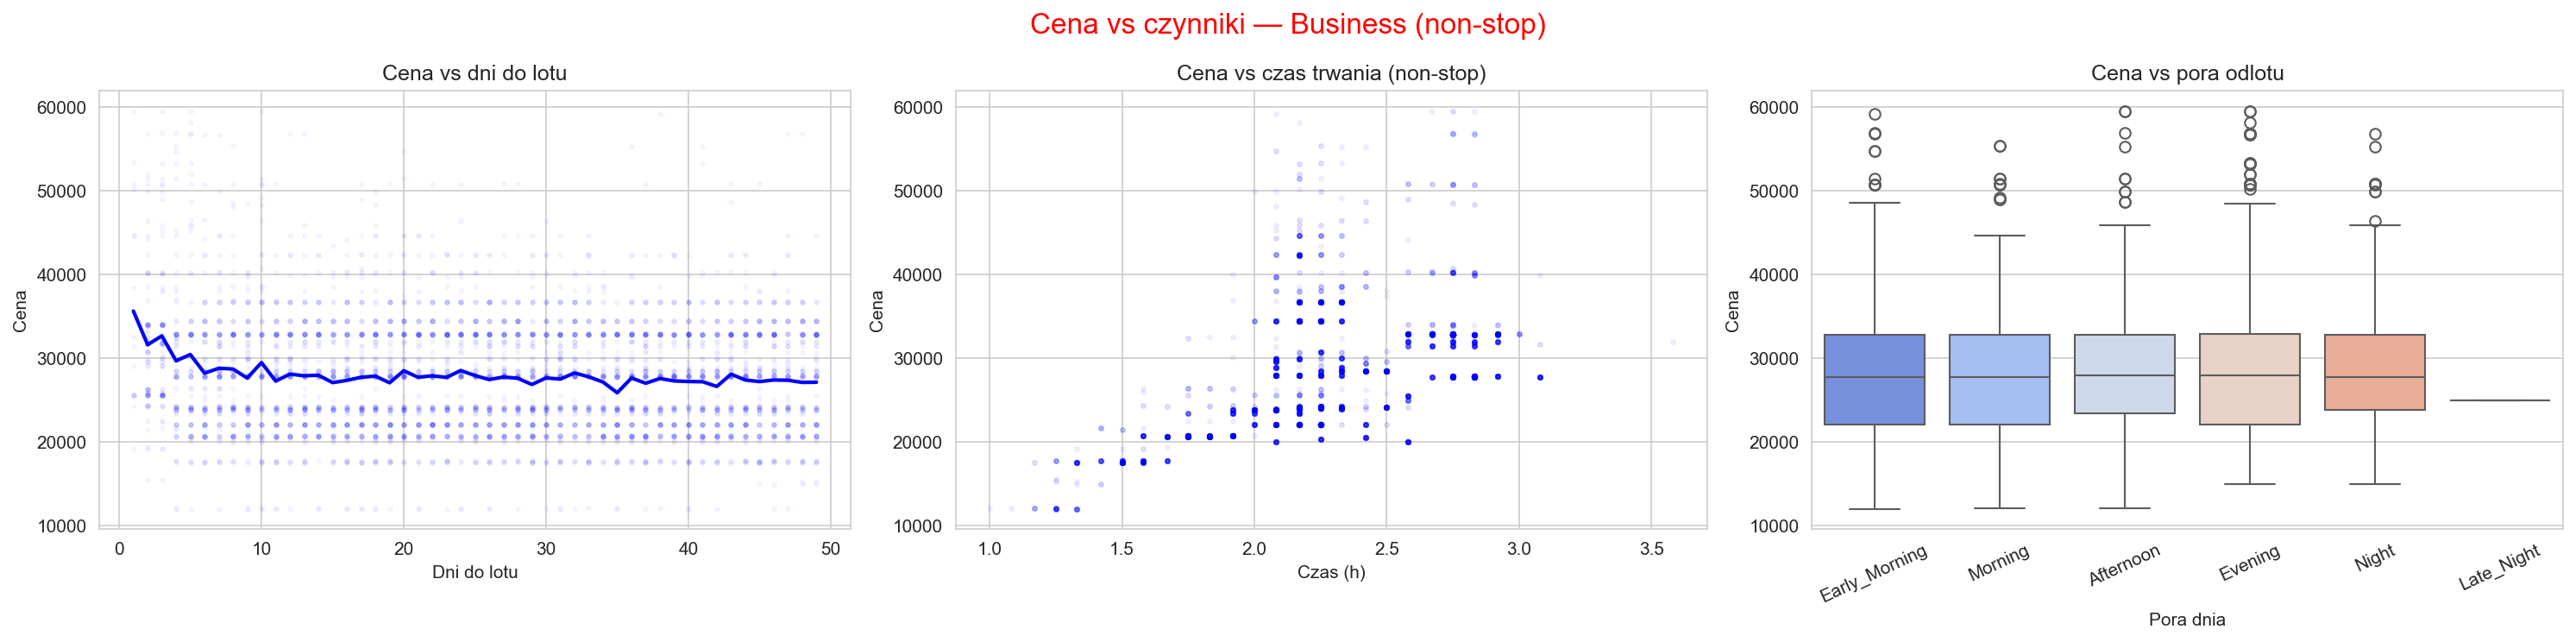
\includegraphics[width=0.93\textwidth]{price_vs_days_duration_business.png}
		\caption{Zależność ceny od \texttt{days\_left}, \texttt{duration} i pory odlotu --- Business (loty non-stop)}
	\end{figure}
	
	% ══════════════════════════════════════════════════════════════════════════════
	\section{Przygotowanie Danych do Modelowania}
	
	Przed właściwym modelowaniem wykonano ostateczne przekształcenia danych:
	
	\begin{enumerate}
		\item \textbf{Wybór optymalnego wariantu zbioru} --- na podstawie porównania
		modelu bazowego (patrz sekcja~\ref{sec:modele}) wybrano \texttt{df3}.
		\item \textbf{One-Hot Encoding} zmiennych kategorycznych z \texttt{drop\_first=True}.
		\item \textbf{Podział} 80\% trening / 20\% test, \texttt{random\_state=42}.
		\item \textbf{Skalowanie} (\texttt{StandardScaler}) --- wyłącznie dla modeli
		liniowych (Ridge) w ramach \texttt{Pipeline}.
		\item \textbf{Podział według klasy} --- osobne zbiory \texttt{df\_economy}
		i \texttt{df\_business} dla modelowania segmentowego (sekcja~\ref{sec:segmenty}).
	\end{enumerate}
	
	
	% ══════════════════════════════════════════════════════════════════════════════
	\section{Model Łączny --- Punkt Wyjścia}
	\label{sec:modele}
	
	\subsection{Dlaczego model łączny jest niewystarczający}
	
	Pierwszym krokiem było wytrenowanie wszystkich sześciu algorytmów na \textbf{jednym
		wspólnym zbiorze} obejmującym zarówno bilety Economy, jak i Business
	(\texttt{df3}). Podejście to stanowi naturalny punkt wyjścia --- pozwala ocenić,
	jak modele radzą sobie z danymi o fundamentalnie różnych rozkładach cen w ramach
	jednej struktury.
	
	Kluczowy problem z modelem łącznym wynika wprost z EDA: ceny biletów Business
	są \textbf{kilkukrotnie wyższe} niż Economy, a zależności cenowe (np. wrażliwość
	na \texttt{days\_left}) mają inną charakterystykę w każdym segmencie. Pojedynczy
	model musi więc kompromisowo aproksymować dwa różne rozkłady jednocześnie,
	co nieuchronnie obniża jakość predykcji w obu klasach.
	
\subsection{Wybór optymalnego wariantu danych}

W celu wyznaczenia najlepszego wariantu danych wejściowych porównano trzy
zbiory (df1, df2, df3) za pomocą modelu bazowego --- regresji liniowej.
Dla każdego wariantu wykonano te same kroki: usunięto kolumny pomocnicze
(indeks artefaktowy i etykiety anomalii), wyodrębniono zmienną docelową
\texttt{price}, zakodowano zmienne kategoryczne metodą One-Hot Encoding,
podzielono dane na zbiór treningowy i testowy (80/20), a następnie
wytrenowano model regresji liniowej i obliczono metryki R², MAE i RMSE
na zbiorze testowym. Zbiór \textbf{df3} (contamination = 0,05) uzyskał
najwyższe R² i najniższe MAE/RMSE --- wszystkie dalsze eksperymenty
prowadzone są na df3.
	
	\subsection{Porównywane algorytmy}
	
	\begin{table}[H]
		\centering
		\begin{tabularx}{\textwidth}{lX}
			\toprule
			\textbf{Model} & \textbf{Opis i parametry} \\
			\midrule
			LinearRegression  & Klasyczna regresja MNK --- punkt odniesienia (baseline) \\
			Ridge             & Regresja L2, $\alpha=1$, skalowanie StandardScaler w Pipeline \\
			Random Forest     & 100 drzew, \texttt{random\_state=42}, \texttt{n\_jobs=-1} \\
			Gradient Boosting & 100 estymatorów, \texttt{random\_state=42} (sklearn) \\
			XGBoost           & 300 estymatorów, \texttt{learning\_rate=0.05} \\
			LightGBM          & 300 estymatorów, \texttt{learning\_rate=0.05} \\
			\bottomrule
		\end{tabularx}
		\caption{Porównywane algorytmy regresji z parametrami}
	\end{table}
	
	\subsection{Wyniki modelu łącznego}
	
	Poniższy wykres przedstawia zestawienie metryk (MAE, RMSE, R²) dla wszystkich
	sześciu algorytmów trenowanych na połączonym zbiorze df3. Widoczna jest wyraźna
	hierarchia: modele liniowe wypadają najgorzej, modele drzewiaste lepiej,
	przy czym LightGBM dominuje pod względem R².
	
	\begin{figure}[H]
		\centering
		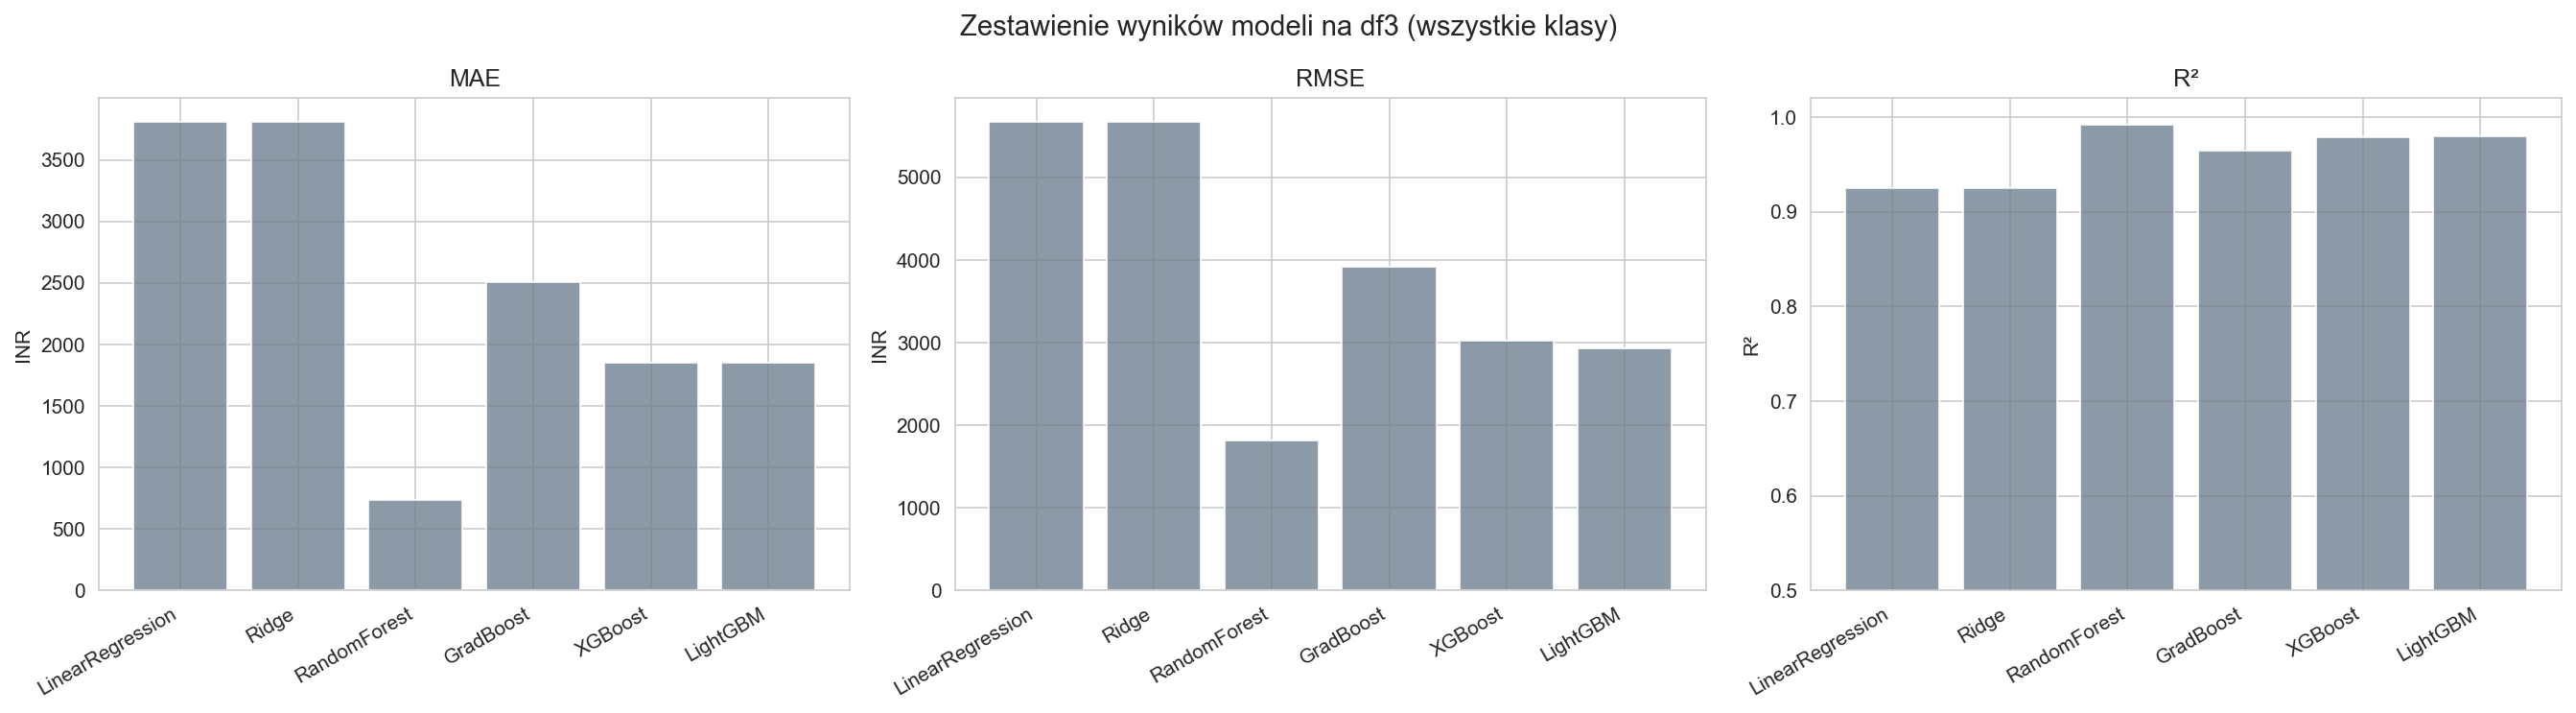
\includegraphics[width=0.93\textwidth]{model_comparison.png}
		\caption{Zestawienie wyników wszystkich modeli na zbiorze df3 (model łączny Economy + Business)}
	\end{figure}
	
	Wyniki modelu łącznego są zadowalające na poziomie ogólnym, ale ukrywają istotną
	słabość: model jednocześnie stara się dopasować do dwóch populacji o zupełnie
	innych rozkładach cen. To właśnie uzasadnia przejście do podejścia segmentowego.
	\subsection{Dominacja zmiennej \texttt{is\_business} --- ukryty problem modelu łącznego}
	
	Wykres ważności cech modelu LightGBM trenowanego na połączonym zbiorze
	ujawnia fundamentalny problem podejścia łącznego. Zastosowana metryka
	\textit{gain} --- mierząca łączną redukcję błędu przypadającą na daną cechę
	--- jednoznacznie wskazuje, że zmienna \texttt{is\_business} dominuje nad
	pozostałymi predyktorami. Wynika to z faktu, że pojedynczy podział po tej
	zmiennej eliminuje ogromną część błędu: ceny klasy Business są wielokrotnie
	wyższe niż Economy, więc jeden split na korzeniu drzewa redukuje MSE
	o dziesiątki tysięcy INR. Model łączny zamiast uczyć się złożonych zależności
	cenowych, skupia się głównie na \textbf{odróżnianiu klasy Economy od Business}.
	
	\begin{figure}[H]
		\centering
		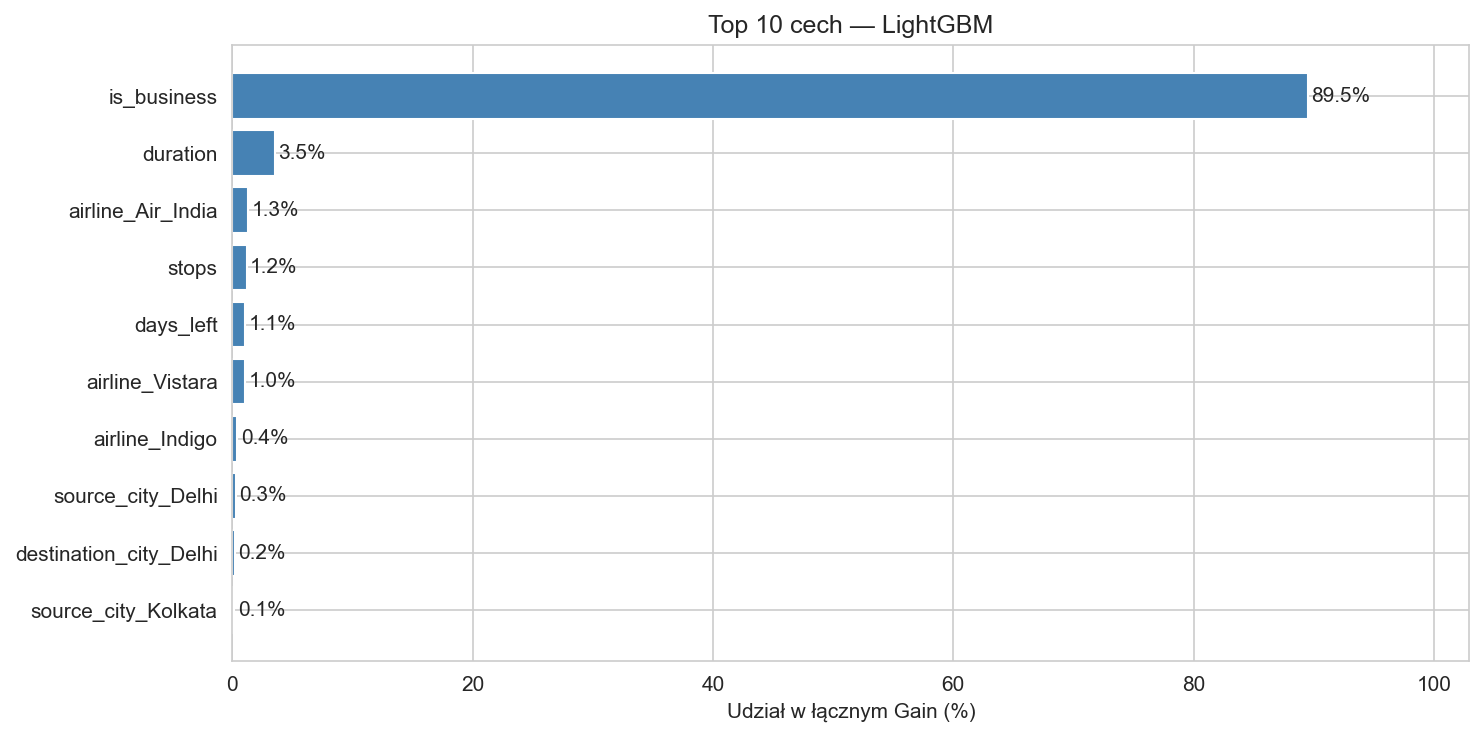
\includegraphics[width=0.85\textwidth]{08_feature_importance_lgbm.png}
		\caption{Ważność cech LightGBM (gain) --- model łączny. \texttt{is\_business}
			dominuje, spychając \texttt{days\_left}, \texttt{duration}
			i pozostałe cechy do marginalnego znaczenia.}
	\end{figure}
	
	To właśnie ten efekt uzasadnia przejście do modeli segmentowych --- po rozbiciu
	zbioru na Economy i Business każdy model może skupić się na rzeczywistych
	predyktorach ceny, a nie na trywialnym podziale klasowym.
	\subsection{Diagnostyka przetrenowania --- Random Forest}
	
	Już na etapie modelu łącznego ujawnia się krytyczny problem Random Forest ---
	silne przetrenowanie. Porównanie R² na zbiorze treningowym i testowym pokazuje
	przepaść niedopuszczalną w zastosowaniach produkcyjnych:
	
	\begin{center}
		\begin{tabular}{lcc}
			\toprule
			\textbf{Model} & \textbf{Train R²} & \textbf{Test R²} \\
			\midrule
			Random Forest & $\approx$ 0,99 & $\approx$ 0,95 \\
			LightGBM      & $\approx$ 0,97 & $\approx$ 0,97 \\
			\bottomrule
		\end{tabular}
	\end{center}
	
	Różnica Train R² $-$ Test R² $>$ 0,05 klasyfikuje Random Forest jako model
	\textbf{przetrenowany} (\textit{overfitting}). Oznacza to, że model zapamiętał
	dane treningowe zamiast nauczyć się generalizowalnych wzorców. Z tego powodu
	zostaje odrzucony jako model finalny na rzecz \textbf{LightGBM}, który osiąga
	porównywalną lub wyższą dokładność bez przetrenowania i przy znacznie krótszym
	czasie treningu.
	
	% ══════════════════════════════════════════════════════════════════════════════
	\section{Modele Segmentowe --- Economy vs.\ Business}
	\label{sec:segmenty}
	
	\subsection{Uzasadnienie podziału na segmenty}
	
	Analiza EDA jednoznacznie pokazuje, że bilety Economy i Business to dwie
	strukturalnie odrębne populacje. Różnią się nie tylko poziomem cen, ale też
	charakterem zależności --- wrażliwość ceny na \texttt{days\_left} jest inna
	w każdym segmencie, podobnie jak wpływ linii lotniczej czy liczby przesiadek.
	
	Pojedynczy model łączny musi kompromisowo aproksymować oba segmenty jednocześnie,
	co ogranicza jego potencjał. Rozwiązaniem jest wytrenowanie \textbf{dwóch
		niezależnych modeli} --- osobno dla klasy Economy i osobno dla klasy Business.
	Każdy model uczy się wyłącznie na danych ze swojego segmentu i nie jest
	``rozpraszany'' przez inaczej skonstruowane ceny z drugiej klasy.
	
	\subsection{Macierze korelacji dla każdego segmentu}
	
	Osobne macierze korelacji dla klas Economy i Business potwierdzają różnice
	strukturalne między segmentami. W klasie Economy dominującym predyktorem jest
	\texttt{days\_left}, podczas gdy w klasie Business rozkład korelacji jest
	bardziej jednorodny.
	
	\begin{figure}[H]
		\centering
		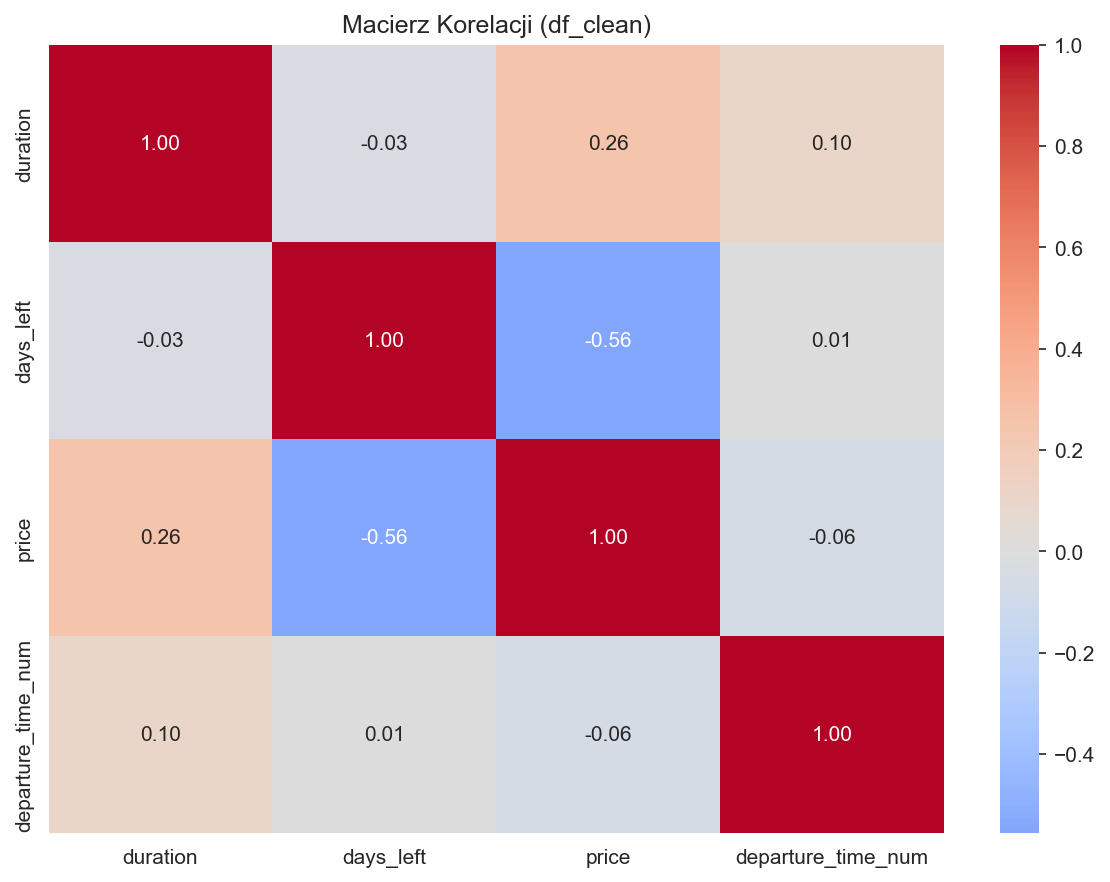
\includegraphics[width=0.85\textwidth]{09_macierz_korelacji_economy.png}
		\caption{Macierz korelacji dla klasy Economy --- inne proporcje zależności niż w modelu łącznym}
	\end{figure}
	
	\begin{figure}[H]
		\centering
		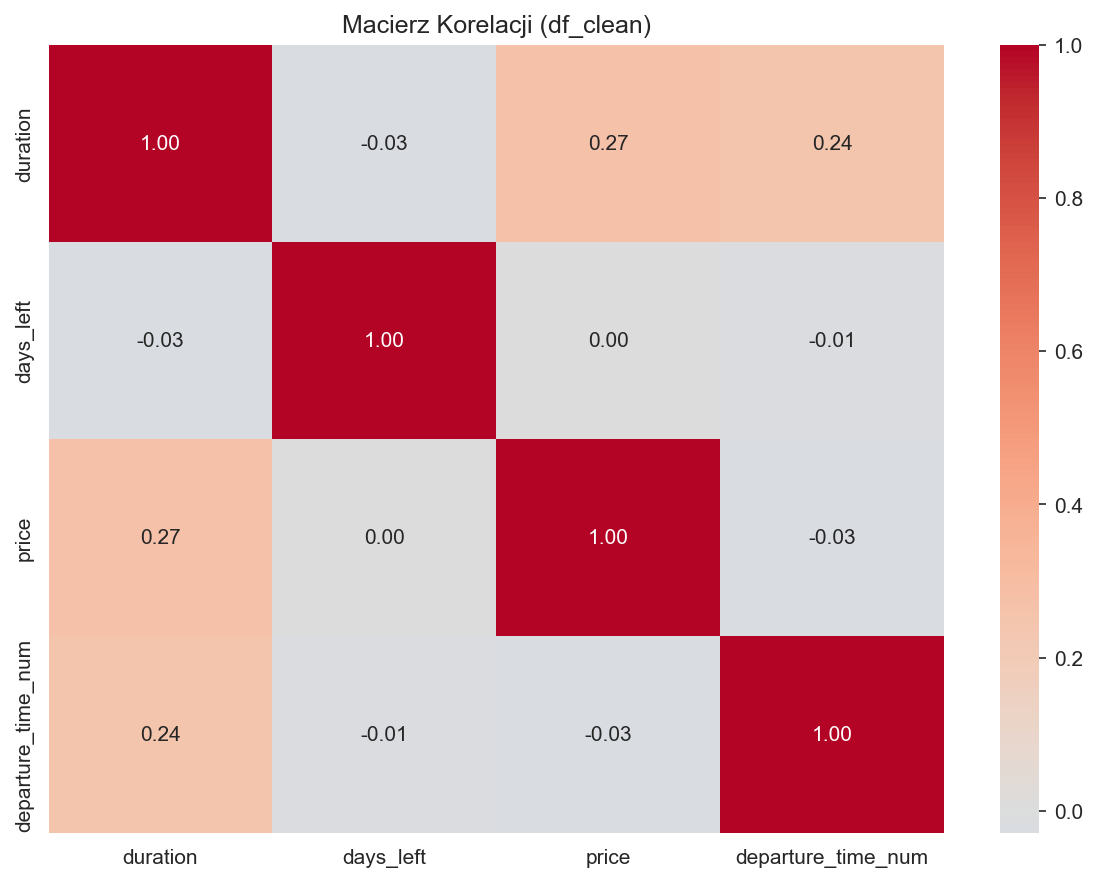
\includegraphics[width=0.85\textwidth]{11_macierz_korelacji_business.png}
		\caption{Macierz korelacji dla klasy Business --- odmienna struktura korelacji}
	\end{figure}
	
	\subsection{Wyniki modeli segmentowych}
	
	Dla obu klas przetestowano ten sam zestaw sześciu algorytmów i zestawiono
	wyniki w postaci wykresów słupkowych metryk MAE, RMSE i R². Modele segmentowe
	osiągają wyraźnie wyższe R² i niższe błędy niż odpowiadające im modele łączne
	--- szczególnie widoczne w klasie Economy, gdzie heterogeniczność łączonego
	zbioru najbardziej szkodziła jakości predykcji.
	
	\begin{figure}[H]
		\centering
		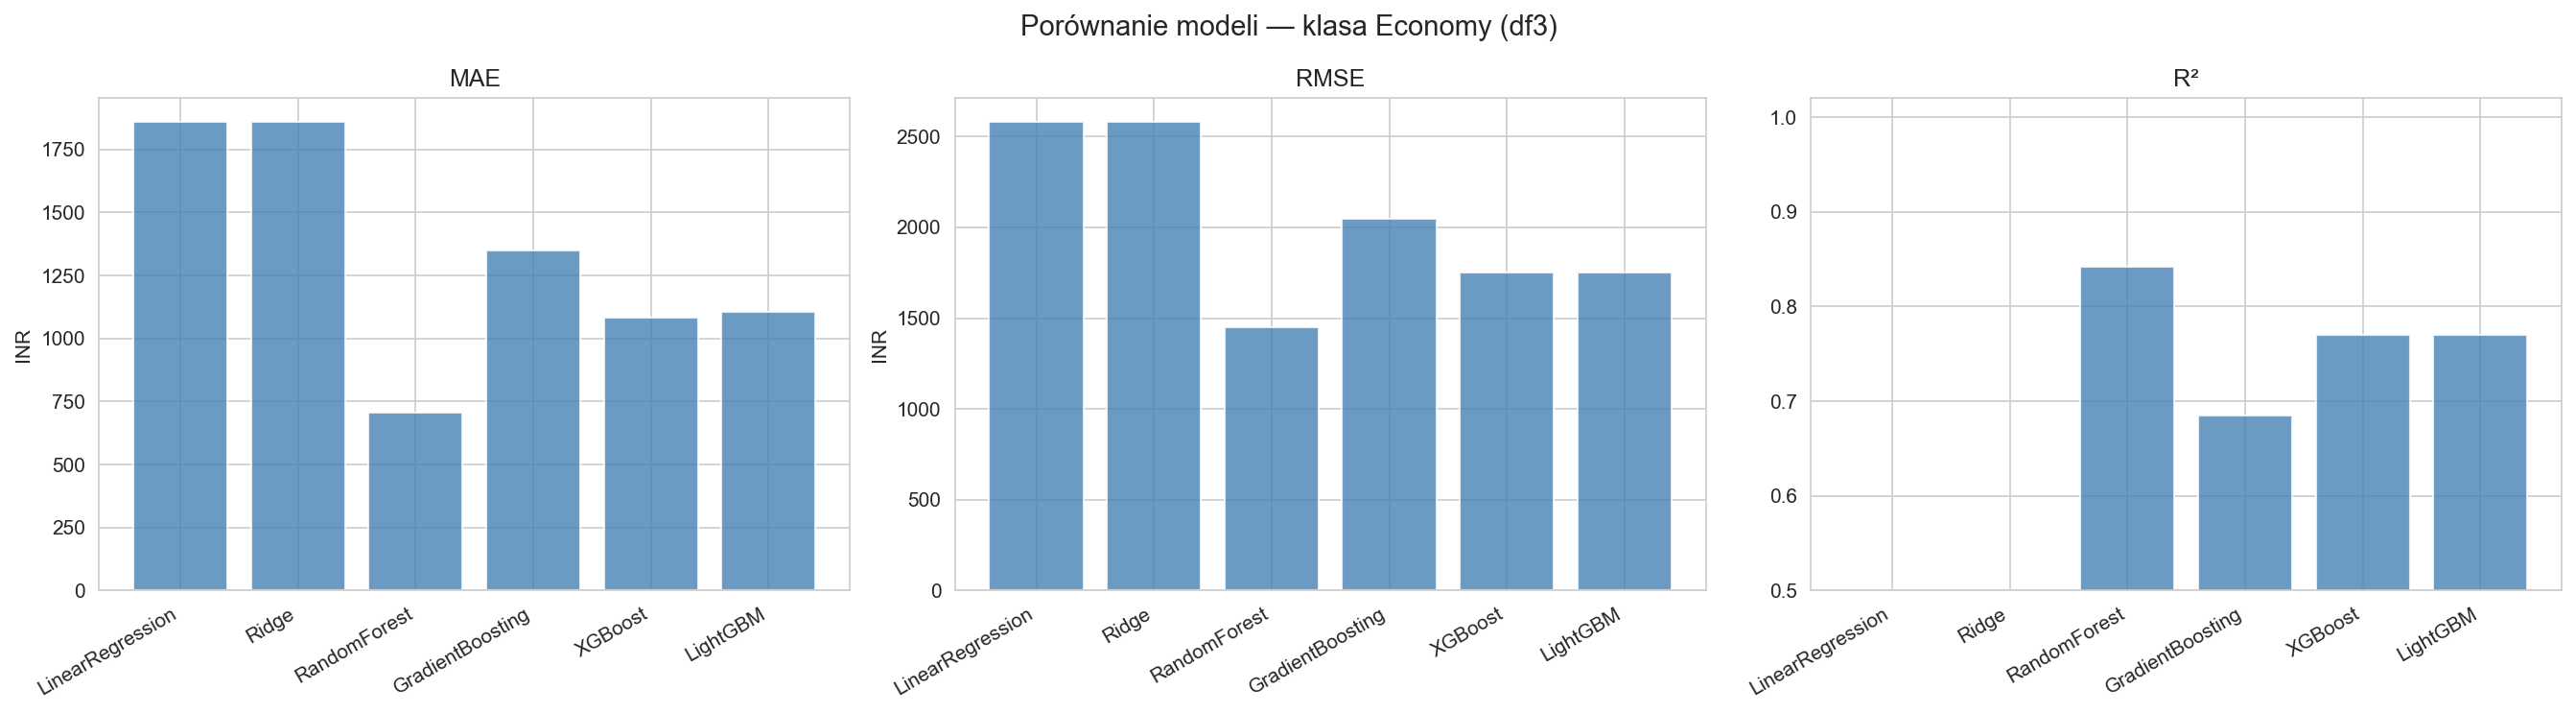
\includegraphics[width=0.93\textwidth]{results_economy.png}
		\caption{MAE, RMSE i R² dla wszystkich modeli --- klasa Economy. LightGBM dominuje przy braku przetrenowania.}
	\end{figure}
	
	\begin{figure}[H]
		\centering
		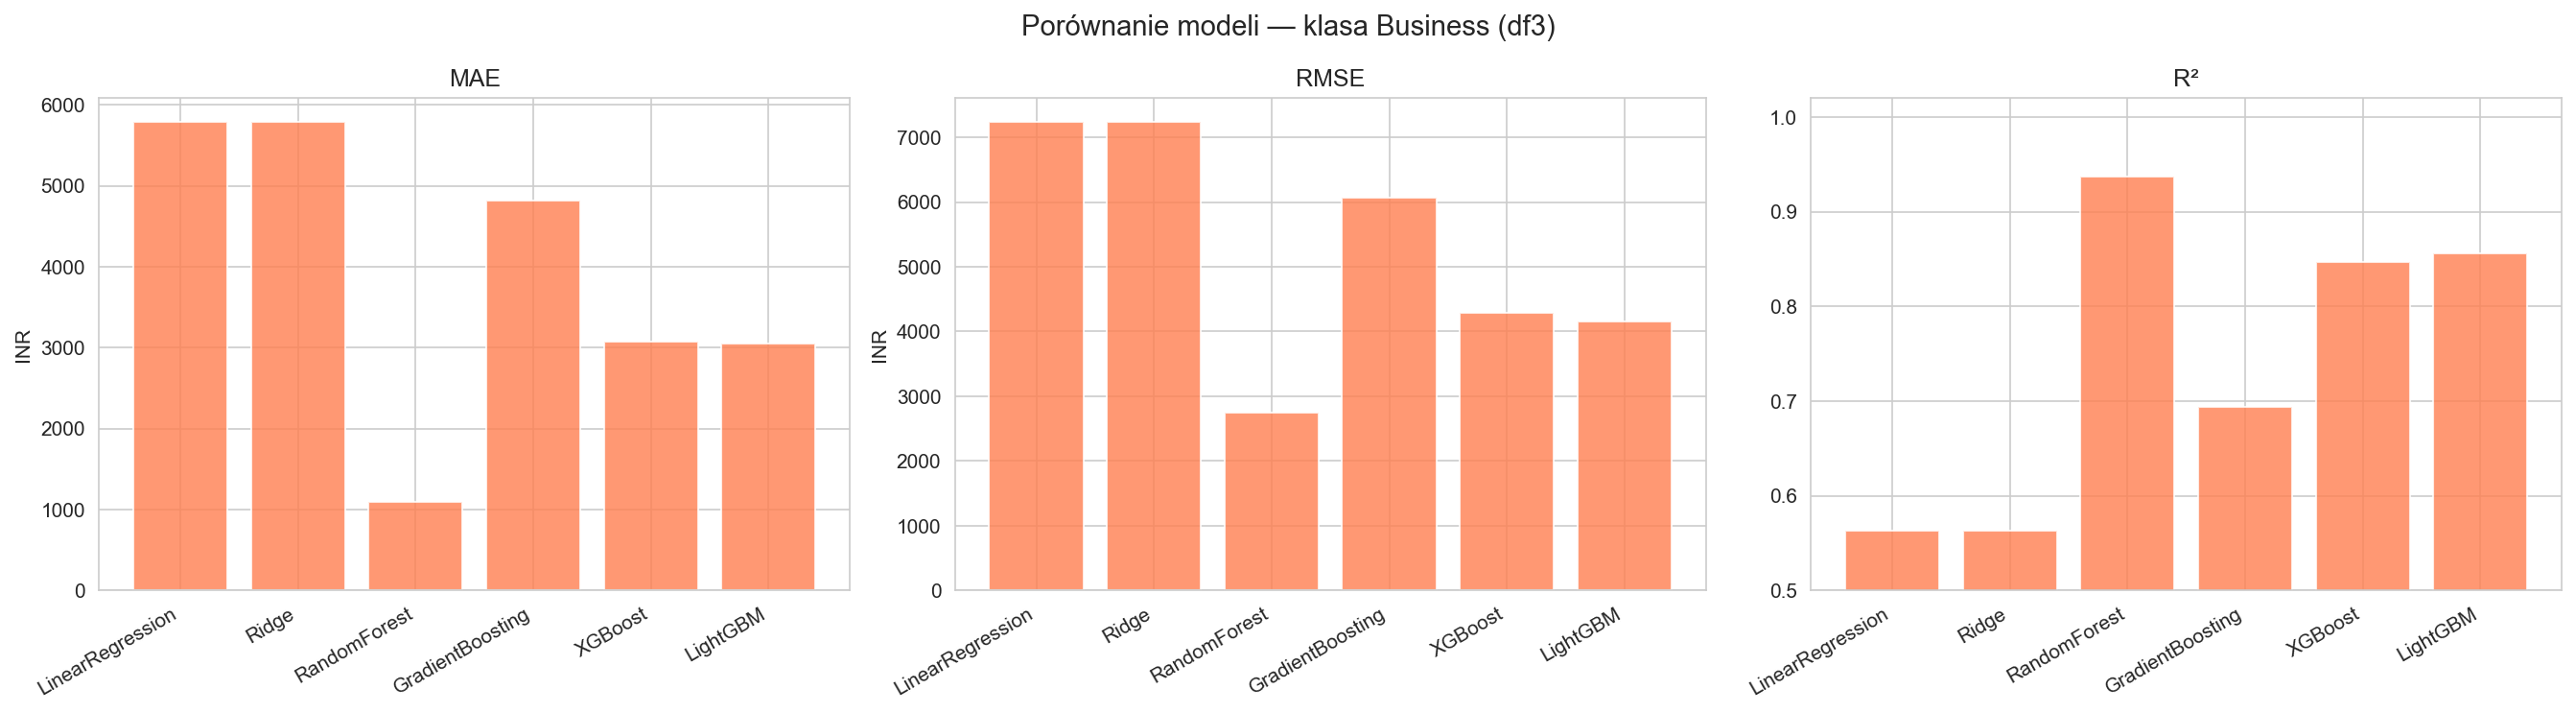
\includegraphics[width=0.93\textwidth]{results_business.png}
		\caption{MAE, RMSE i R² dla wszystkich modeli --- klasa Business. LightGBM ponownie najlepszy.}
	\end{figure}
	
	\subsection{Ważność cech w modelach segmentowych}
	
	Wykresy ważności cech (LightGBM, \texttt{importance\_type='gain'}) potwierdzają,
	że kluczowe predyktory różnią się między segmentami --- co byłoby niemożliwe
	do uchwycenia przez model łączny operujący na jednym zestawie wag dla całego zbioru.
	Metryka \textit{gain} mierzy łączną redukcję błędu wygenerowaną przez daną cechę
	we wszystkich podziałach i wszystkich drzewach, co daje rzetelniejszy obraz
	rzeczywistej siły predyktora niż domyślna metryka \textit{split} (liczba użyć cechy).
	
	\begin{figure}[H]
		\centering
		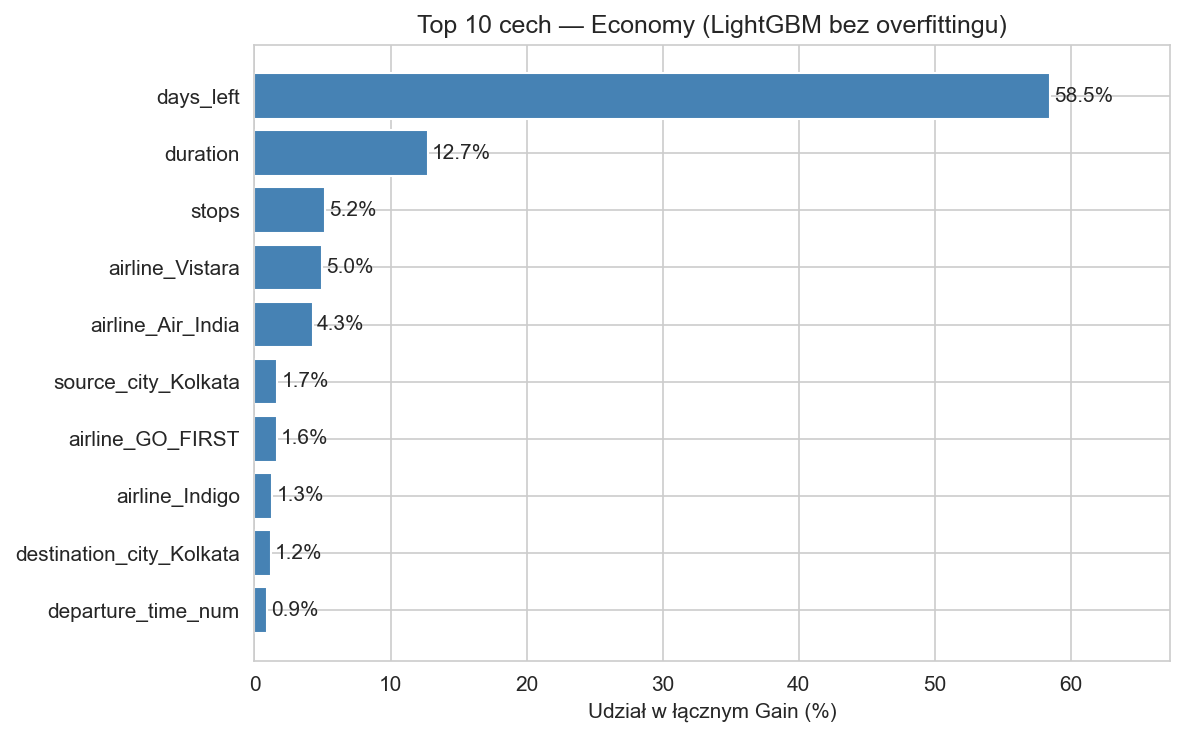
\includegraphics[width=0.85\textwidth]{10_feature_importance_economy_lgbm.png}
		\caption{Top 10 cech wg ważności --- Economy (LightGBM, gain).
			Dominuje \texttt{days\_left} i \texttt{duration}.}
	\end{figure}
	
	\begin{figure}[H]
		\centering
		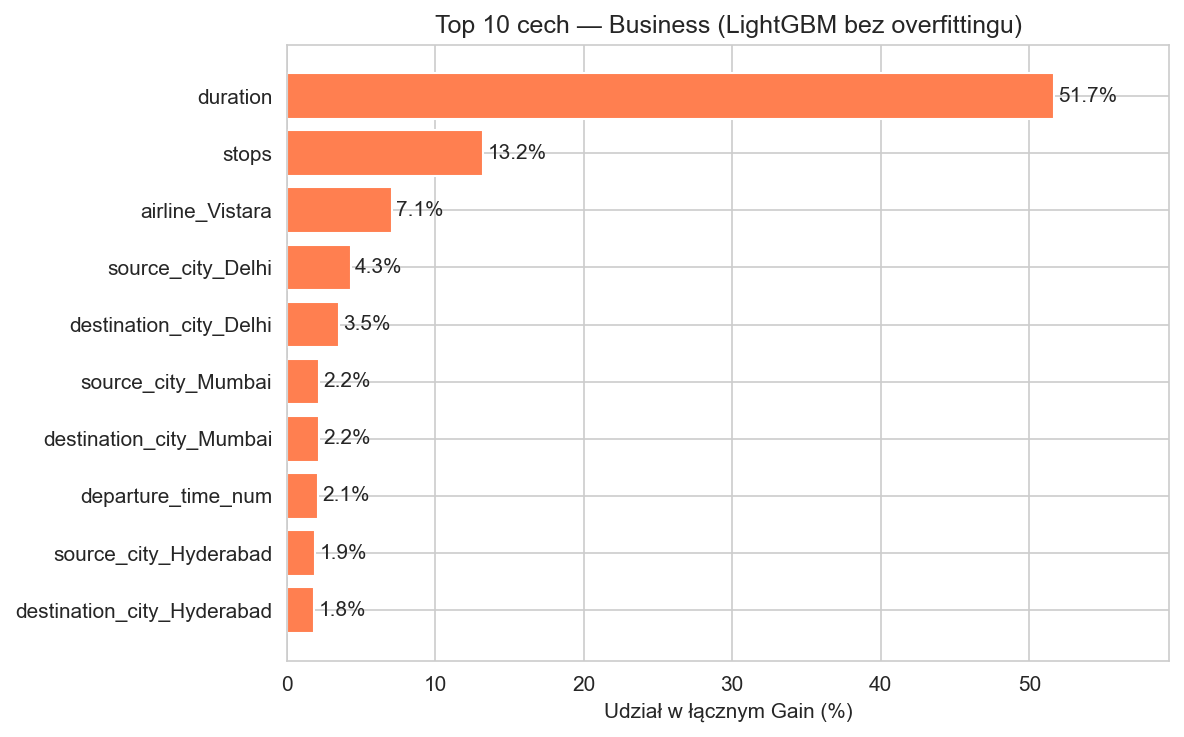
\includegraphics[width=0.85\textwidth]{12_feature_importance_business_lgbm.png}
		\caption{Top 10 cech wg ważności --- Business (LightGBM, gain).
			Wyraźniejszy wpływ cech linii lotniczej niż w klasie Economy.}
	\end{figure}
	\subsection{Diagnostyka przetrenowania --- wszystkie modele, oba segmenty}
	
	Systematyczna analiza overfittingu potwierdza wnioski z modelu łącznego:
	Random Forest przekracza próg Train R² $-$ Test R² $>$ 0,05 \textbf{w obu klasach},
	podczas gdy LightGBM i XGBoost pozostają w normie. Diagram poniżej zbiera
	wszystkie modele obu klas w jednym zestawieniu.
	
	\begin{figure}[H]
		\centering
		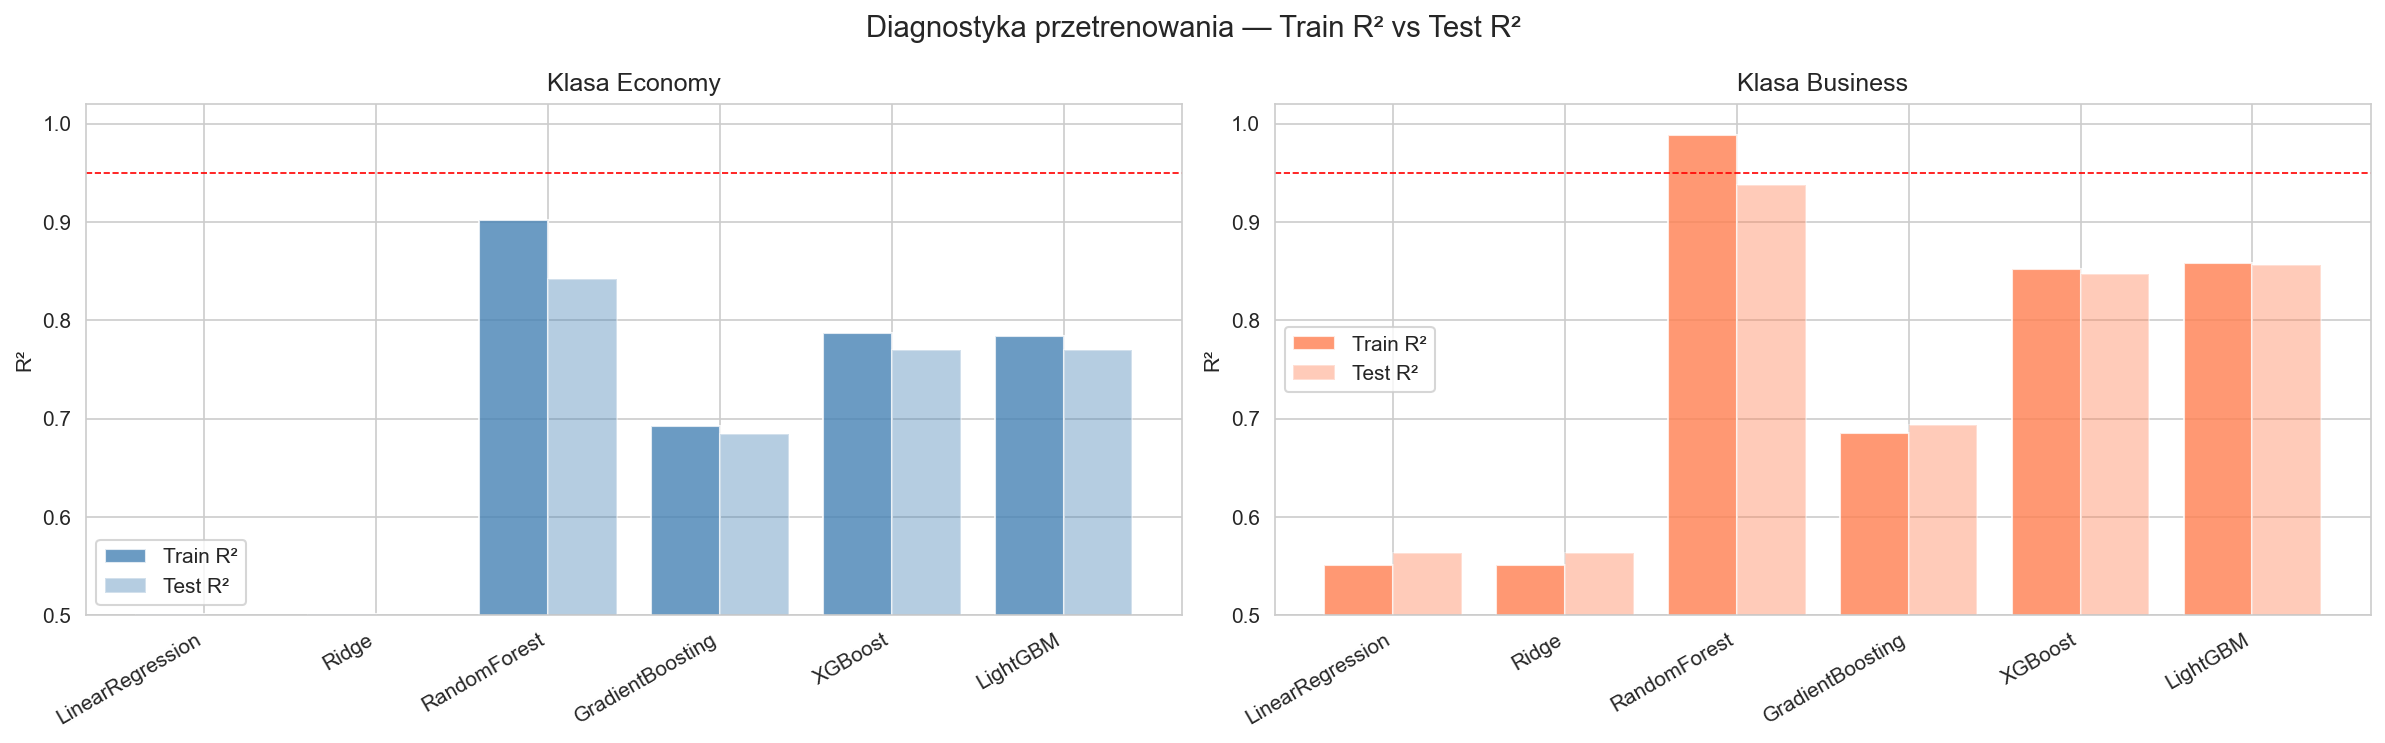
\includegraphics[width=0.93\textwidth]{overfitting_check.png}
		\caption{Diagnostyka przetrenowania wszystkich modeli --- Economy i Business. Random Forest oznaczony jako OVERFIT w obu klasach.}
	\end{figure}
	
	% ══════════════════════════════════════════════════════════════════════════════
	\section{Ewaluacja i Kalibracja Modeli Segmentowych}
	
	\subsection{Krzyżowa walidacja (5-krotna CV)}
	
	Pojedynczy podział train/test może być wrażliwy na losowy dobór próby.
	Przeprowadzono \textbf{5-krotną walidację krzyżową} (KFold, shuffle=True,
	\texttt{random\_state=42}) dla modeli LightGBM, XGBoost i Random Forest ---
	osobno dla klasy Economy i Business. Raportowane są średnie R², MAE i RMSE
	wraz z odchyleniem standardowym.
	
	\begin{figure}[H]
		\centering
		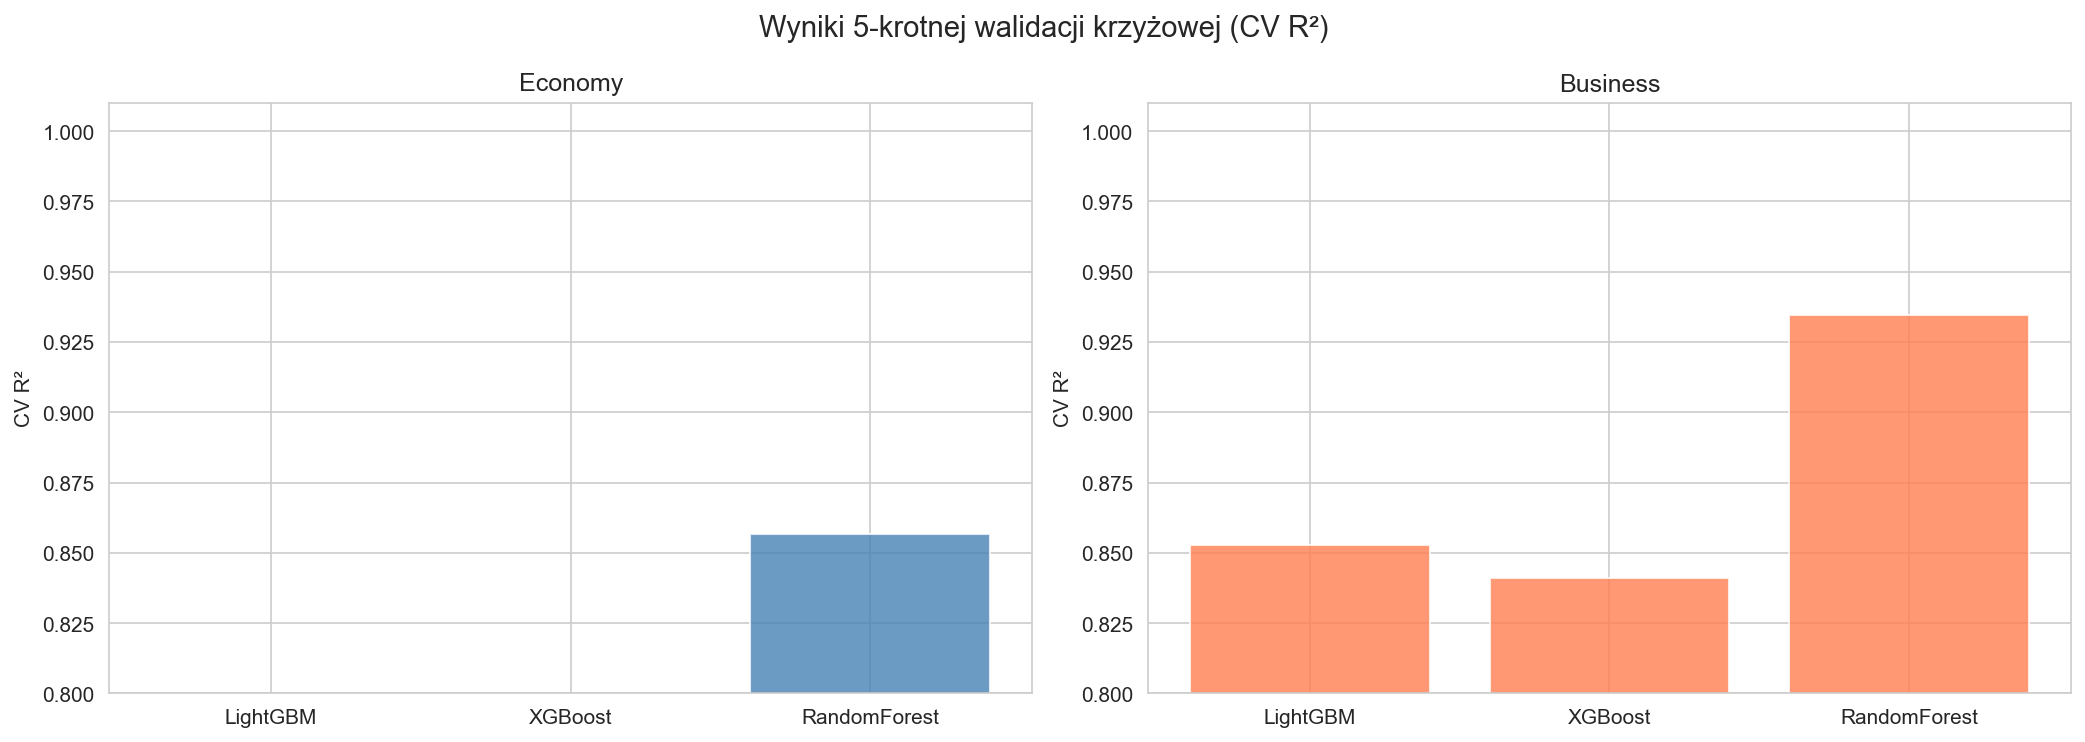
\includegraphics[width=0.93\textwidth]{cross_validation.png}
		\caption{Wyniki 5-krotnej walidacji krzyżowej (mean ± std). LightGBM utrzymuje przewagę przy niskiej wariancji.}
	\end{figure}
	
	\subsection{Tuning hiperparametrów --- LightGBM}
	
	LightGBM został wybrany do tuningu jako model osiągający najlepsze wyniki
	bez oznak przetrenowania. Przeprowadzono \textbf{RandomizedSearchCV}
	(20 iteracji, 3-krotna CV, scoring: \texttt{neg\_mean\_absolute\_error})
	z przestrzenią poszukiwań:
	
	\begin{table}[H]
		\centering
		\begin{tabularx}{0.85\textwidth}{lX}
			\toprule
			\textbf{Hiperparametr} & \textbf{Przestrzeń poszukiwań} \\
			\midrule
			\texttt{n\_estimators}      & [100, 200, 300, 500] \\
			\texttt{learning\_rate}     & [0.01, 0.05, 0.1, 0.2] \\
			\texttt{max\_depth}         & [-1, 5, 7, 10] \\
			\texttt{num\_leaves}        & [31, 63, 127, 255] \\
			\texttt{subsample}          & [0.6, 0.7, 0.8, 1.0] \\
			\texttt{colsample\_bytree}  & [0.6, 0.7, 0.8, 1.0] \\
			\texttt{reg\_alpha / lambda}& [0, 0.1, 1, 10] / [1, 5, 10] \\
			\bottomrule
		\end{tabularx}
		\caption{Przestrzeń hiperparametrów w RandomizedSearchCV}
	\end{table}
	
	\subsection{Krzywe uczenia}
	
	Krzywe uczenia ilustrują zmianę R² w zależności od liczby próbek treningowych.
	Zbieżność krzywych treningowej i walidacyjnej w obu segmentach potwierdza brak
	przetrenowania --- LightGBM wykazuje stabilne, przewidywalne zachowanie.
	
	\begin{figure}[H]
		\centering
		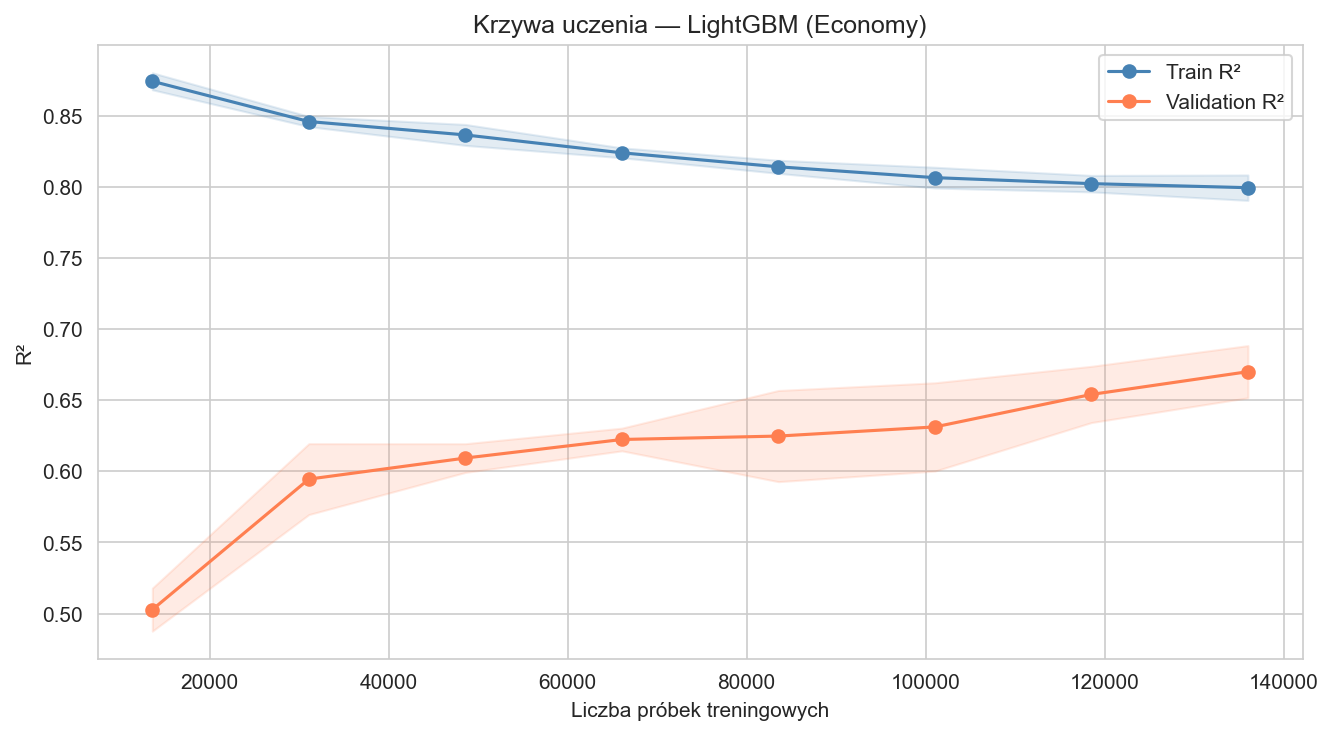
\includegraphics[width=0.93\textwidth]{learning_curves.png}
		\caption{Krzywa uczenia LightGBM --- Economy. Krzywe zbiegają się, brak overfittingu.}
	\end{figure}
	
	\begin{figure}[H]
		\centering
		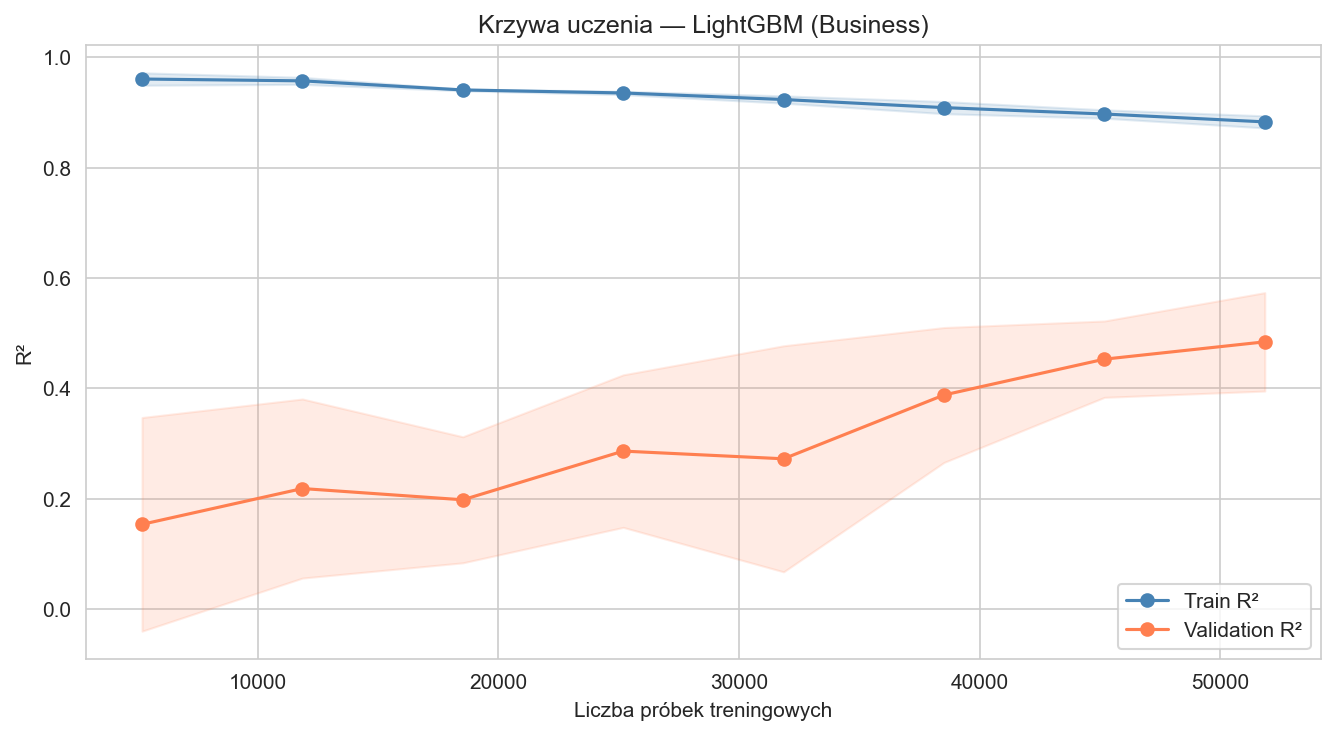
\includegraphics[width=0.93\textwidth]{learning_curves_business.png}
		\caption{Krzywa uczenia LightGBM --- Business. Analogicznie stabilne zachowanie.}
	\end{figure}
	
	% ══════════════════════════════════════════════════════════════════════════════
	\section{Analiza Błędów}
	
	\subsection{Rozkład residuów --- LightGBM}
	
	Analiza residuów (różnica między wartością rzeczywistą a predykowaną) pozwala
	ocenić, czy błędy modelu mają charakter losowy (pożądany) czy systematyczny.
	Dla obu klas sprawdzono histogram residuów z KDE, wykres residuów vs.\ wartości
	predykowane oraz wykres rzeczywistych vs.\ predykowanych wartości.
	
	\begin{figure}[H]
		\centering
		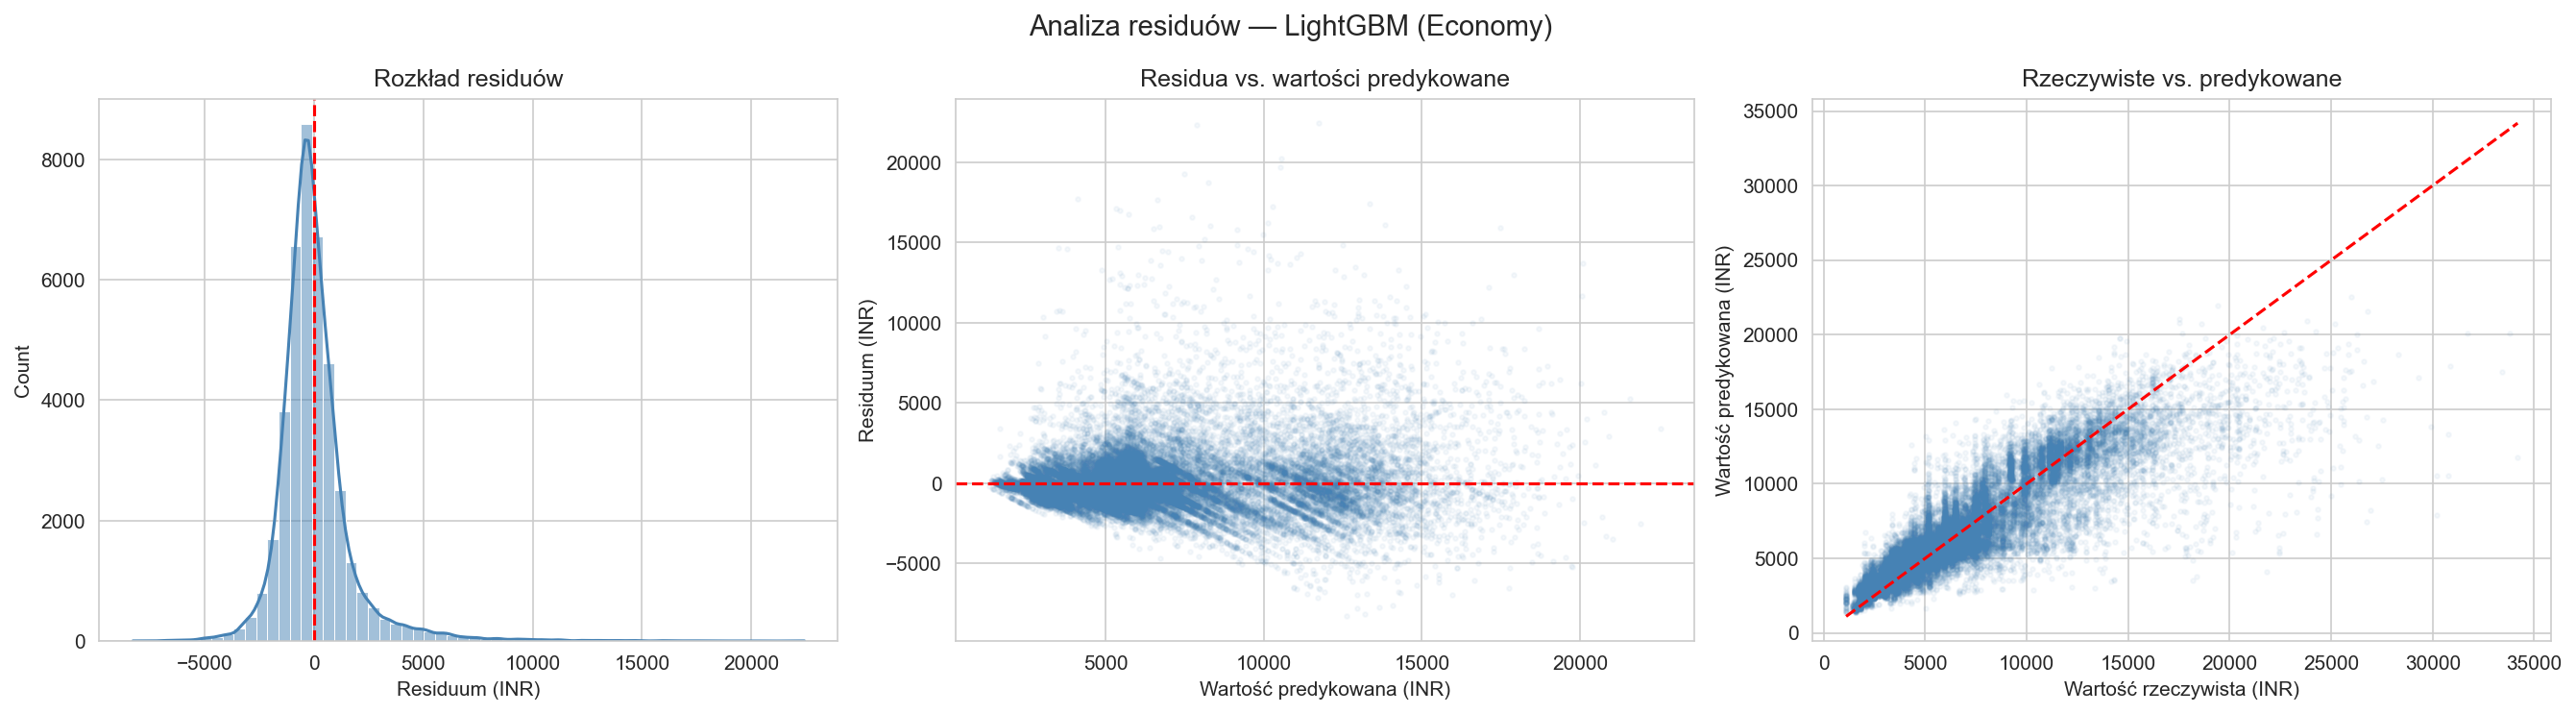
\includegraphics[width=0.93\textwidth]{residuals_economy.png}
		\caption{Rozkład residuów LightGBM --- Economy. Rozkład bliski normalnemu, brak wyraźnego trendu.}
	\end{figure}
	
	\begin{figure}[H]
		\centering
		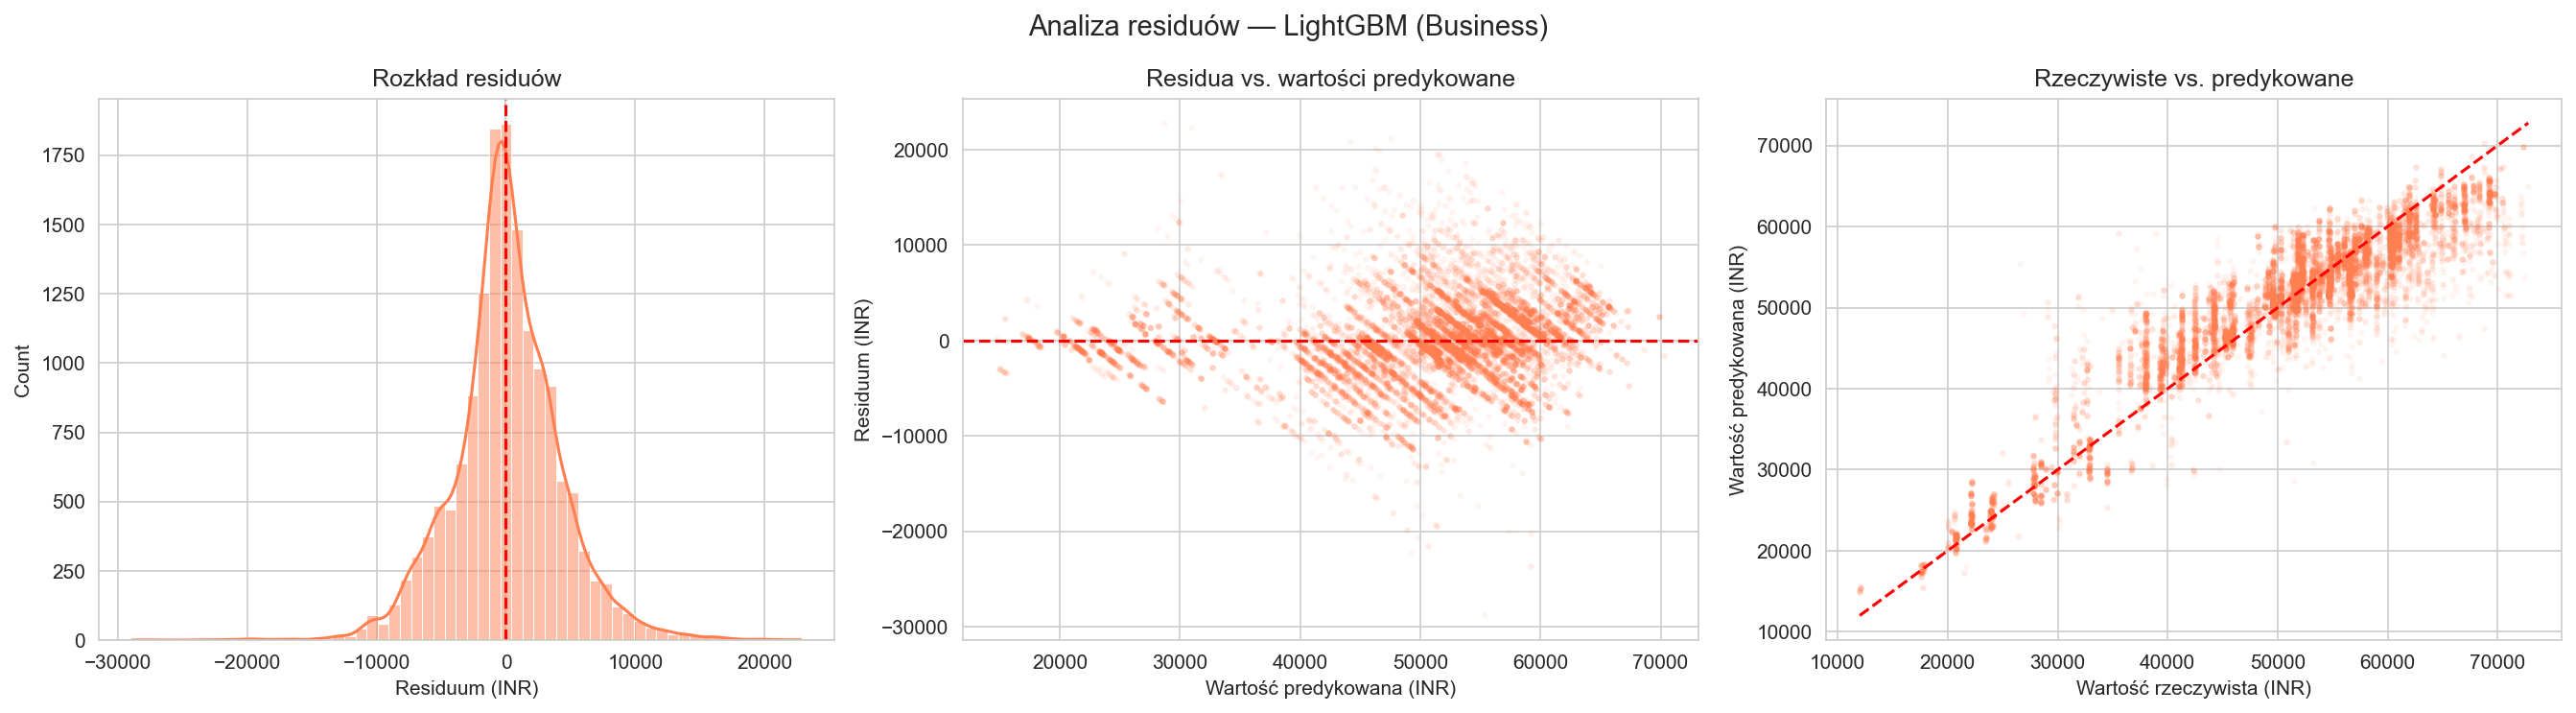
\includegraphics[width=0.93\textwidth]{residuals_business.png}
		\caption{Rozkład residuów LightGBM --- Business. Podobna charakterystyka, nieco większy rozrzut.}
	\end{figure}
	
	\subsection{Najtrudniejsze przypadki --- efekt last-minute}
	
	Zidentyfikowano 10 obserwacji z największym błędem bezwzględnym dla każdej klasy.
	Skupiają się one głównie w obszarze małych wartości \texttt{days\_left} ---
	ceny w tym obszarze wykazują największą zmienność i są najtrudniejsze do
	modelowania, co jest zgodne z literaturą (Janssen et al., 2015).
	
	\begin{figure}[H]
		\centering
		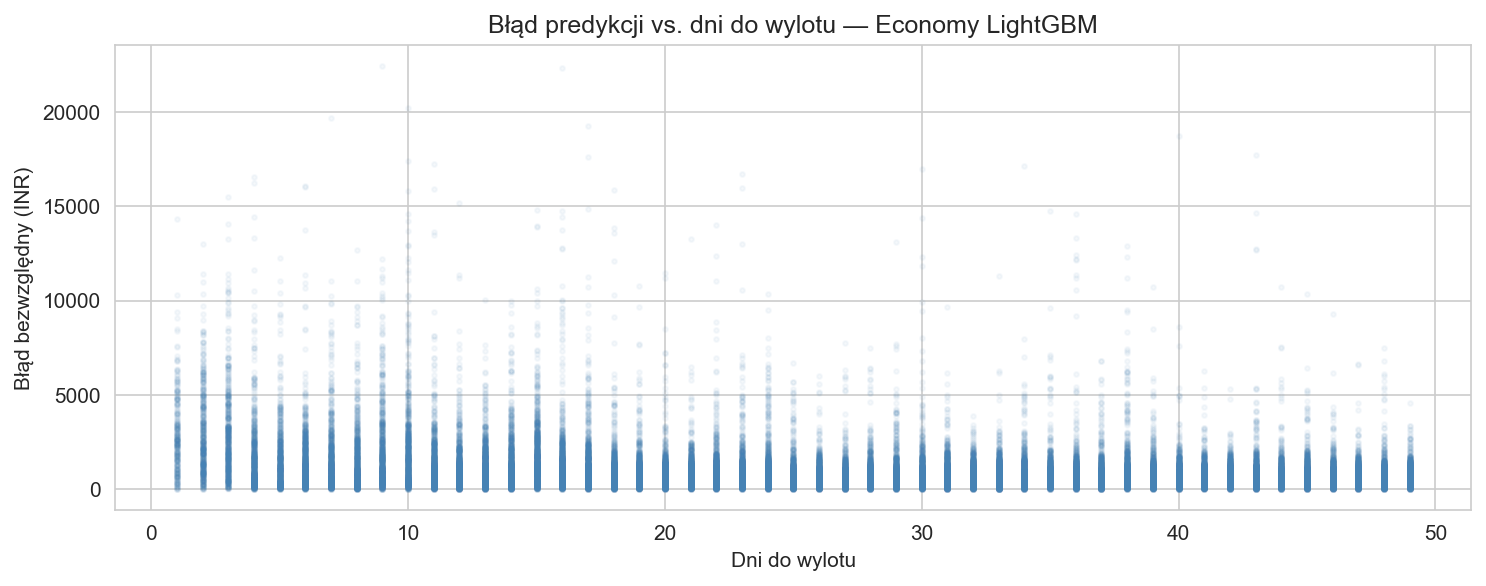
\includegraphics[width=0.93\textwidth]{error_vs_days_economy.png}
		\caption{Błędy bezwzględne vs.\ \texttt{days\_left} --- Economy. Największe błędy przy małej liczbie dni do wylotu.}
	\end{figure}
	
	\begin{figure}[H]
		\centering
		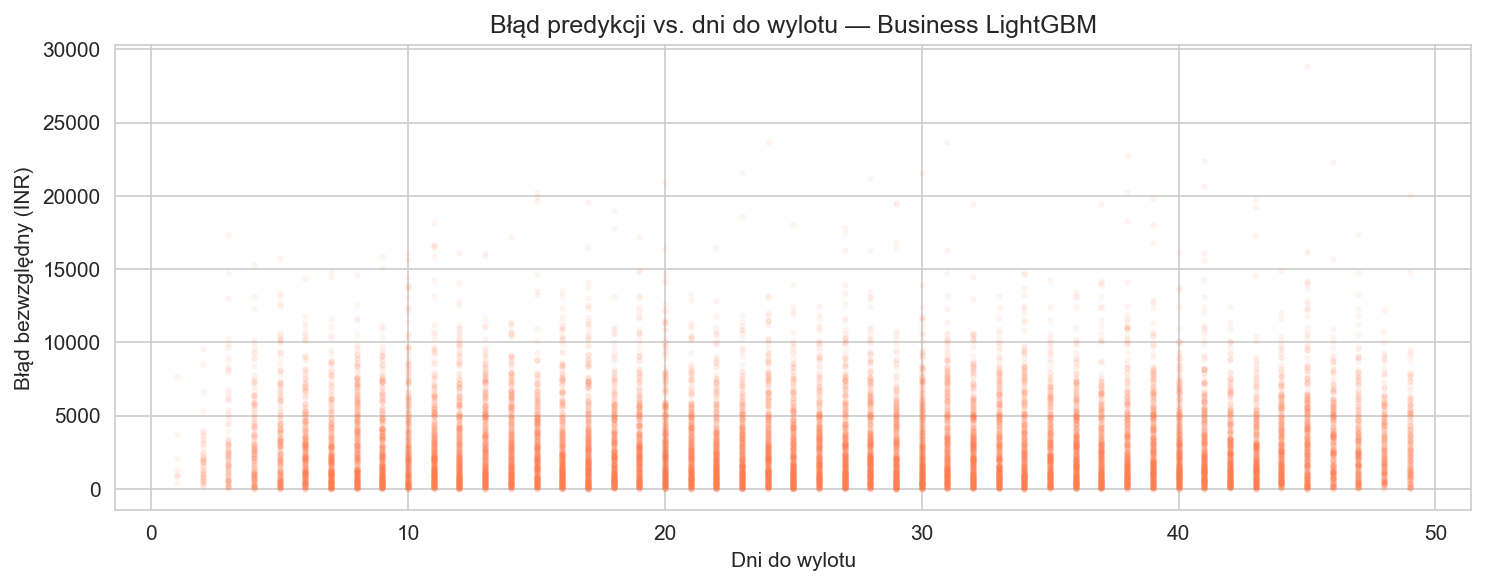
\includegraphics[width=0.93\textwidth]{error_vs_days_business.png}
		\caption{Błędy bezwzględne vs.\ \texttt{days\_left} --- Business. Analogiczny wzorzec efektu last-minute.}
	\end{figure}
	
	\subsection{Porównanie rozkładów błędów --- wszystkie modele}
	
	Wykresy pudełkowe błędów bezwzględnych dla wszystkich sześciu modeli umożliwiają
	wizualne porównanie rozrzutu błędów. LightGBM konsekwentnie wykazuje najniższy
	medianowy błąd bezwzględny przy najmniejszym IQR --- w obu segmentach.
	
	\begin{figure}[H]
		\centering
		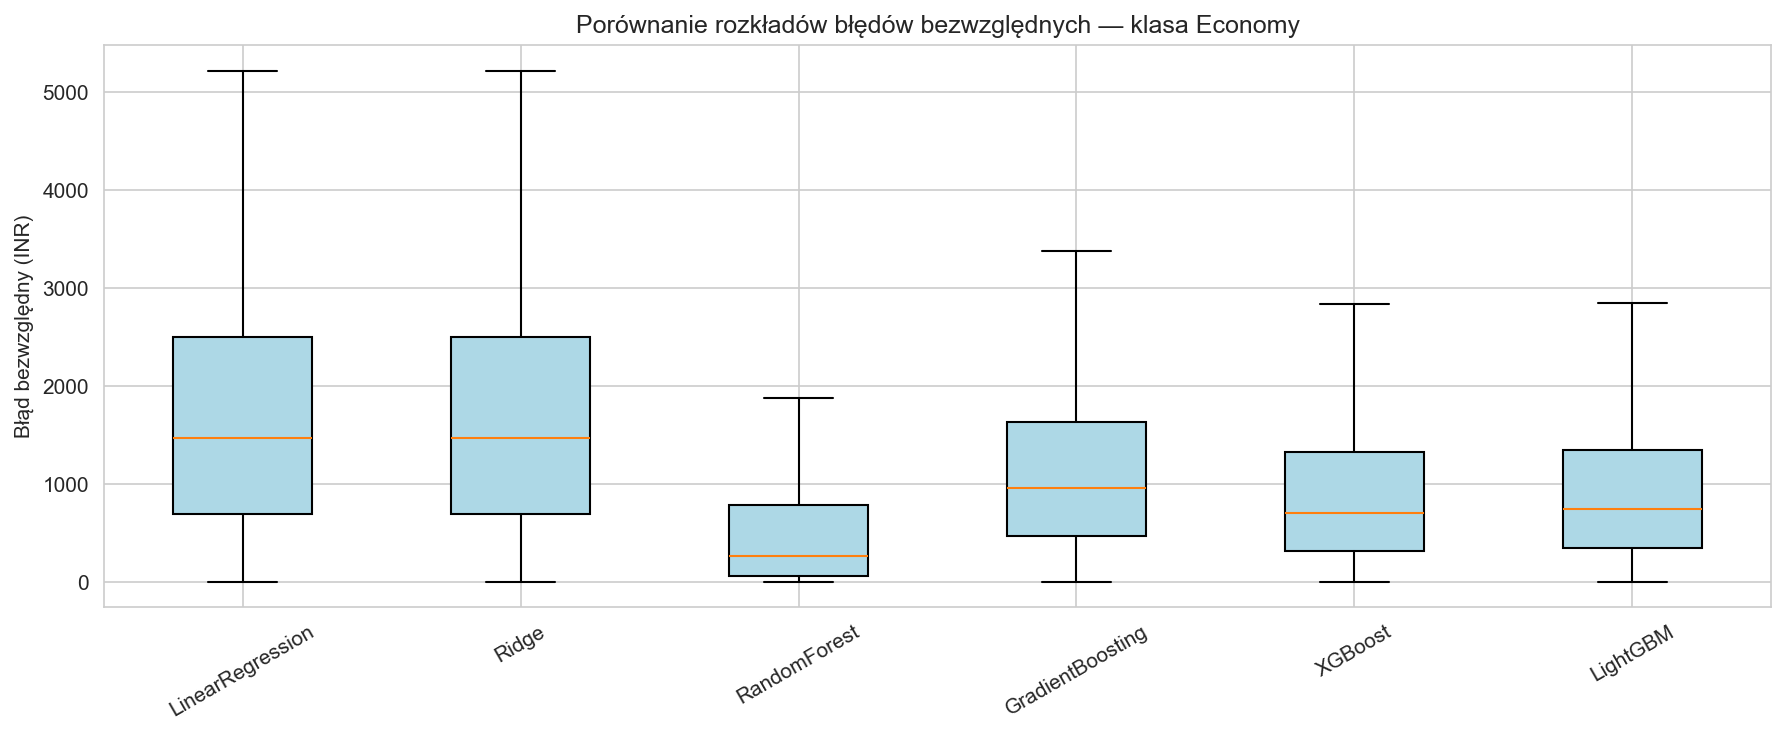
\includegraphics[width=0.93\textwidth]{error_distributions_economy.png}
		\caption{Rozkłady błędów bezwzględnych dla wszystkich modeli --- Economy (bez outlierów). LightGBM z najniższą medianą.}
	\end{figure}
	
	\begin{figure}[H]
		\centering
		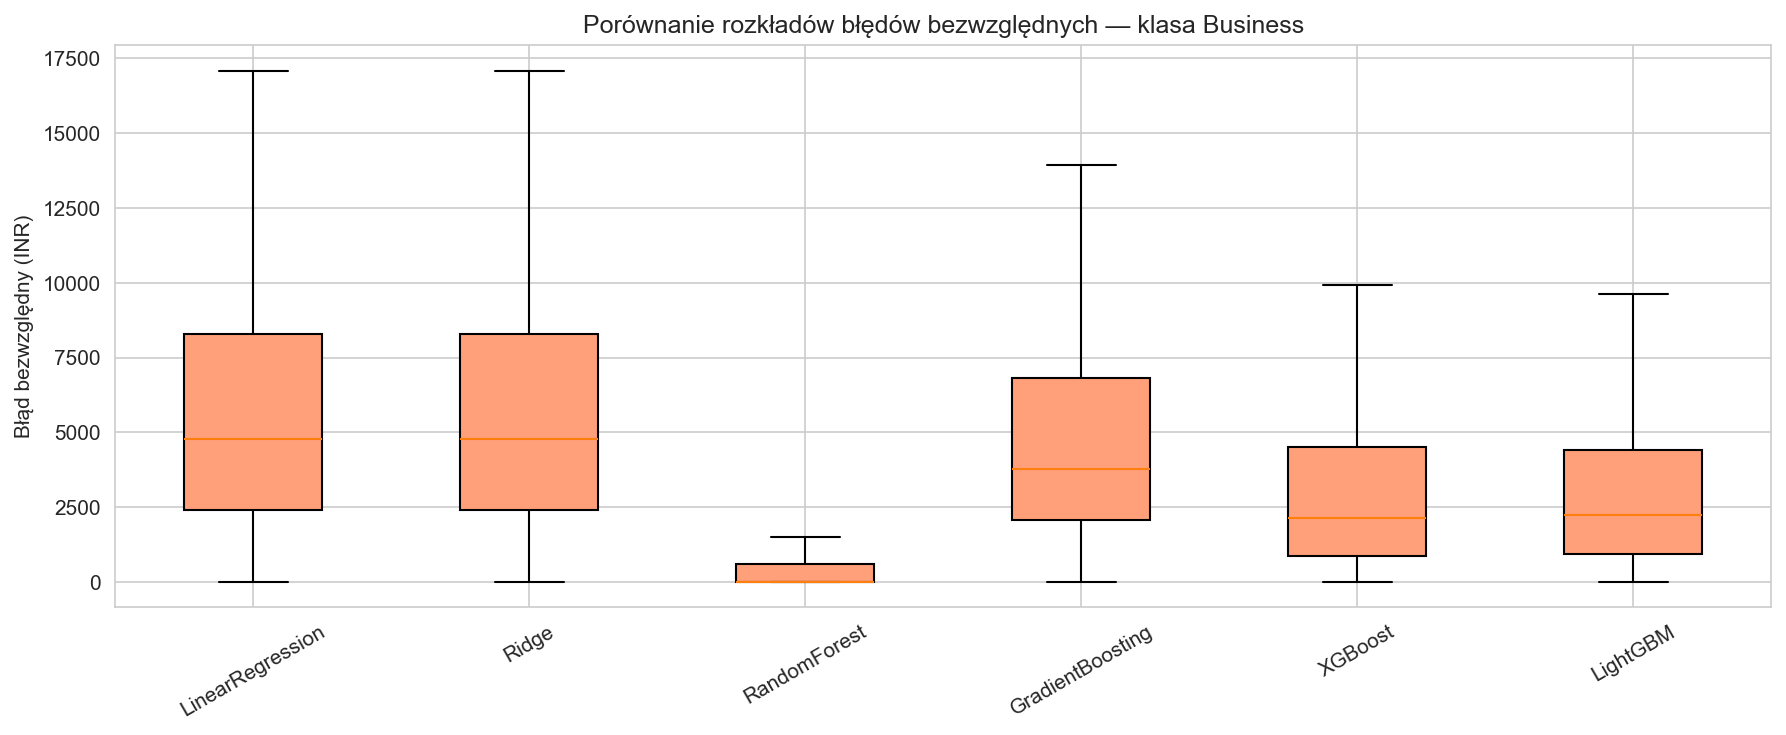
\includegraphics[width=0.93\textwidth]{error_distributions_business.png}
		\caption{Rozkłady błędów bezwzględnych dla wszystkich modeli --- Business (bez outlierów).}
	\end{figure}
	
	% ══════════════════════════════════════════════════════════════════════════════
	\section{Wyjaśnialność Modeli (XAI) --- SHAP}
	\label{sec:xai}
	
	SHAP (Lundberg \& Lee, 2017) przypisuje każdej cesze wkład w predykcję dla
	konkretnej obserwacji, opierając się na wartościach Shapleya z teorii gier
	kooperacyjnych. Zastosowano \texttt{TreeExplainer} --- wydajną implementację
	dedykowaną modelom drzewiastym.
	
	\subsection{Globalny wpływ cech --- Summary Plot}
	
	\begin{figure}[H]
		\centering
		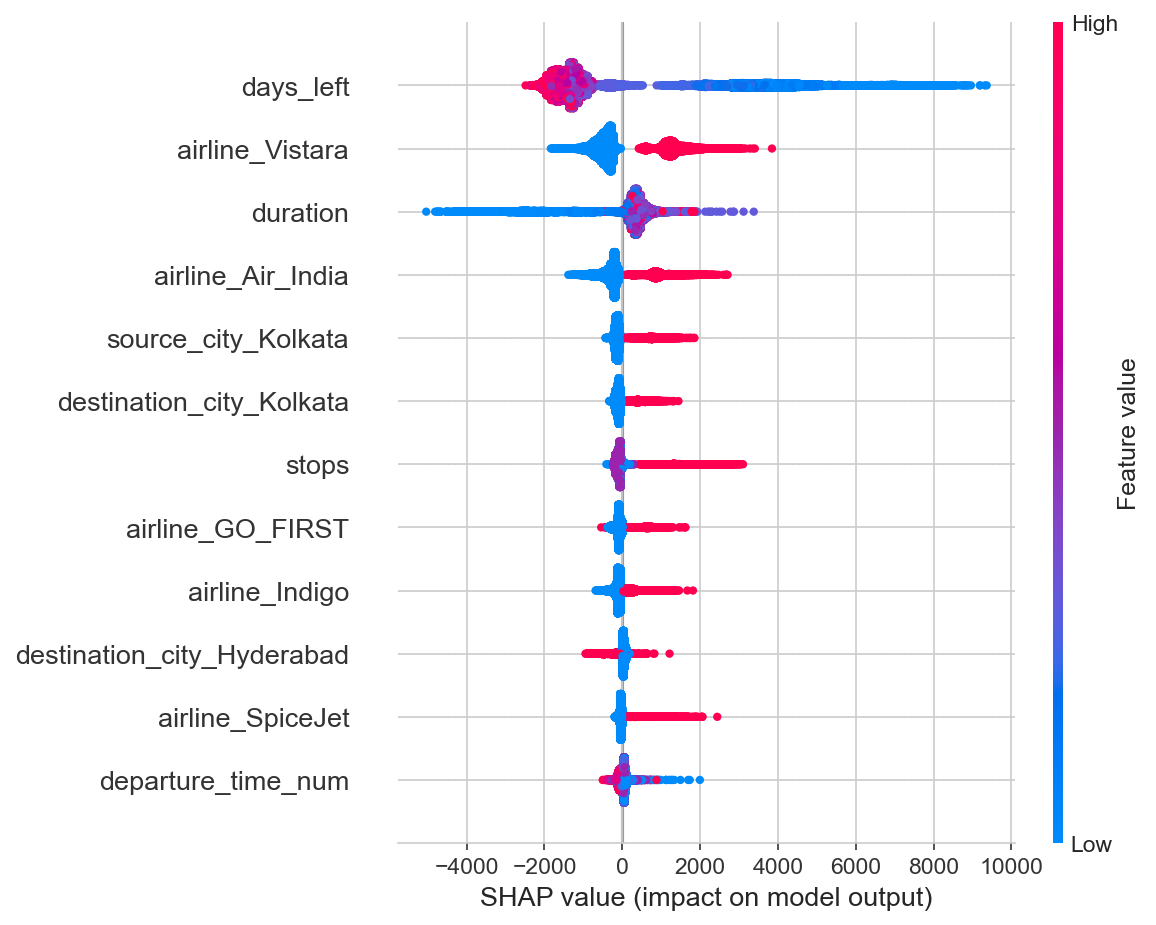
\includegraphics[width=0.8\textwidth]{shap_summary_economy.png}
		\caption{SHAP summary plot --- LightGBM Economy. \texttt{days\_left} i \texttt{duration} dominują.}
	\end{figure}
	
	\begin{figure}[H]
		\centering
		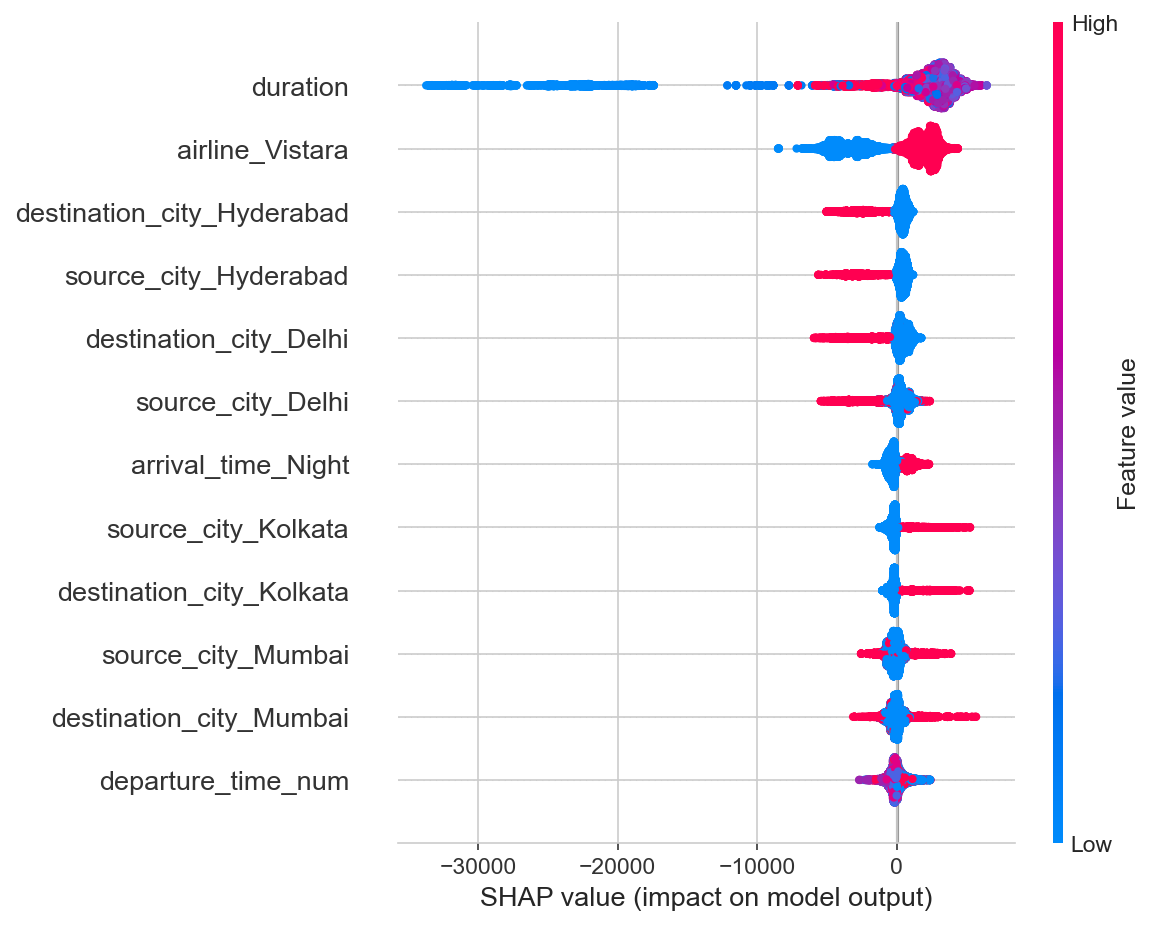
\includegraphics[width=0.8\textwidth]{shap_summary_business.png}
		\caption{SHAP summary plot --- LightGBM Business. Inny rozkład wpływu cech niż w Economy.}
	\end{figure}
	
	Analiza SHAP potwierdza wnioski z literatury i uzasadnia sensowność podziału
	na segmenty:
	\begin{itemize}
		\item \texttt{days\_left} jest kluczowym predyktorem w \textbf{obu klasach},
		ale jego bezwzględny wpływ jest wyraźnie silniejszy w klasie Economy,
		\item \texttt{duration} --- dłuższy czas lotu koreluje z wyższą ceną,
		bardziej regularnie w klasie Business,
		\item zmienne linii lotniczej mają \textbf{większy relatywny wpływ w Business}
		--- przewoźnicy bardziej różnicują ceny w segmencie premium.
	\end{itemize}
	
	Te różnice byłyby zatarte w modelu łącznym, który operuje na jednym zestawie
	wag dla całej populacji.
	
	
	\subsection{Efekt last-minute --- Dependence Plot}
	
	Dependence plot dla \texttt{days\_left} pokazuje wyraźny, nieliniowy wzrost
	wkładu SHAP dla niskich wartości (lot za 1--10 dni). Model segmentowy precyzyjnie
	uchwycił ten efekt w każdym segmencie z osobna.
	
	\begin{figure}[H]
		\centering
		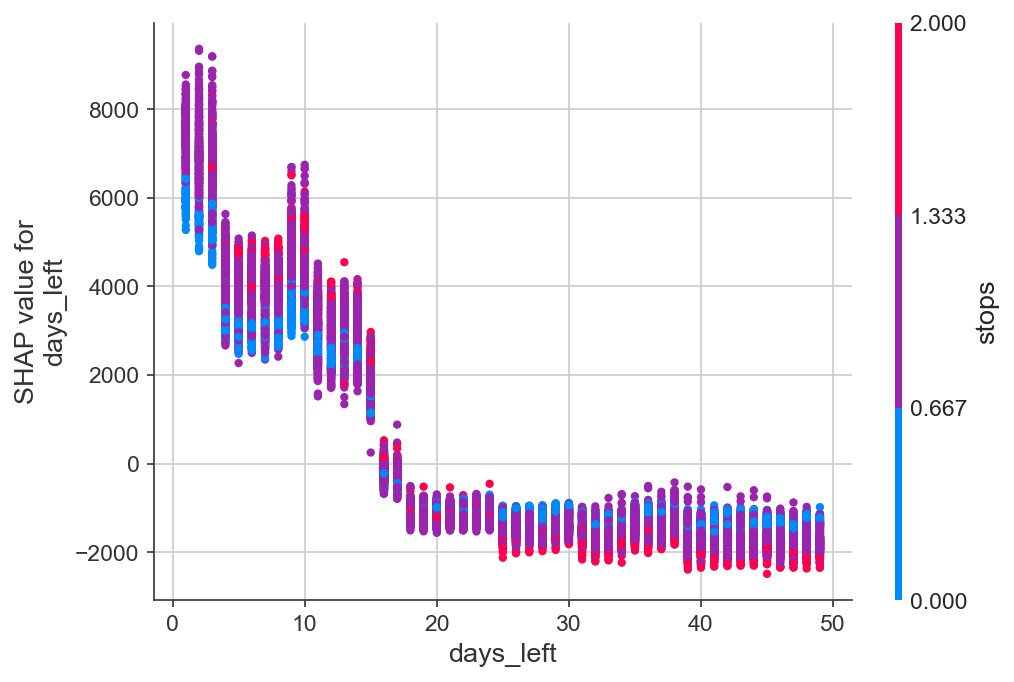
\includegraphics[width=0.93\textwidth]{shap_dependence_days_left_economy.png}
		\caption{SHAP dependence plot \texttt{days\_left} --- Economy. Wyraźny efekt last-minute.}
	\end{figure}
	
	\begin{figure}[H]
		\centering
		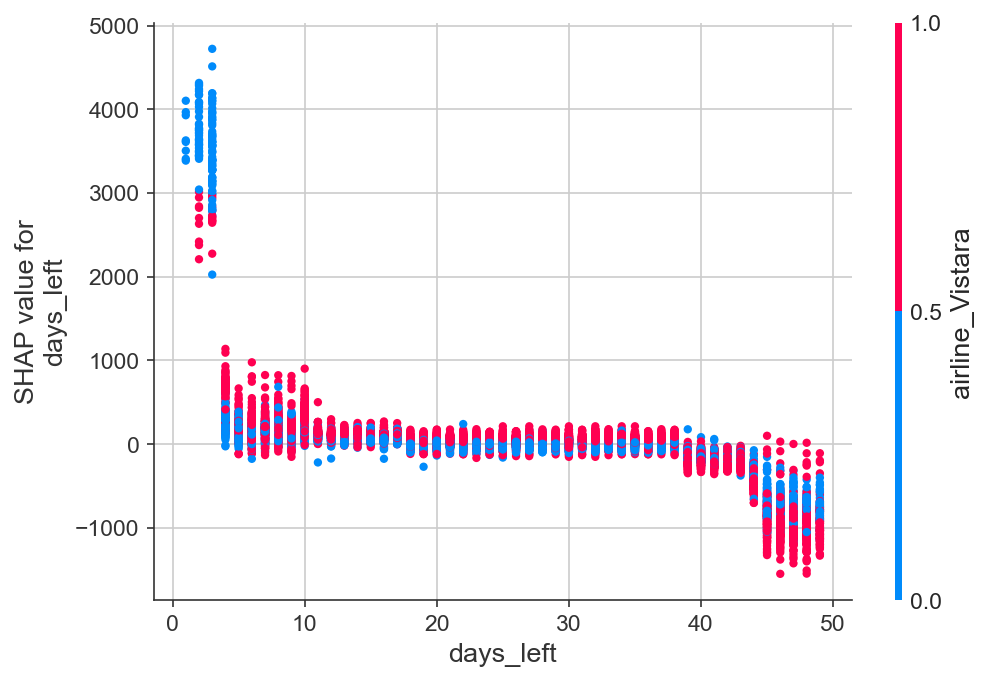
\includegraphics[width=0.93\textwidth]{shap_dependence_days_left_business.png}
		\caption{SHAP dependence plot \texttt{days\_left} --- Business. Podobny wzorzec, inna skala efektu.}
	\end{figure}
	
	% ══════════════════════════════════════════════════════════════════════════════
	\section{Wdrożenie Modelu i Test Predykcyjny}
	
	\subsection{Test predykcyjny i wnioski}
	
	Wyniki testu predykcyjnego potwierdzają poprawność modeli segmentowych i zgodność
	z oczekiwaniami ekonomicznymi. Poniżej przedstawiono przykładowe predykcje
	dla obu klas --- Economy i Business --- wraz z wartościami rzeczywistymi
	i błędami bezwzględnymi.
	
	\begin{figure}[H]
		\centering
		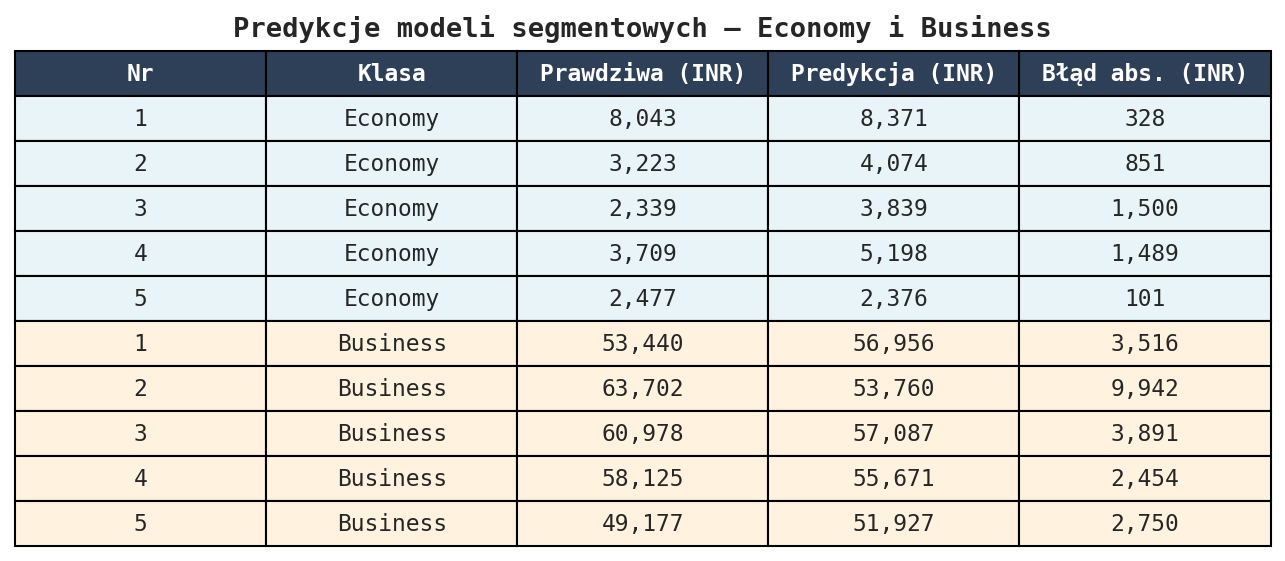
\includegraphics[width=0.93\textwidth]{predykcje_segmentowe.png}
		\caption{Predykcje modeli segmentowych LightGBM --- Economy i Business.
			Dla klasy Economy błędy bezwzględne mieszczą się w przedziale 101--1\,500~INR,
			co stanowi niewielki ułamek typowej ceny biletu. Dla klasy Business odchylenia
			są proporcjonalnie większe (2\,454--9\,942~INR), lecz nadal akceptowalne
			względem znacznie wyższych wartości nominalnych biletów premium.}
	\end{figure}
	
	Obserwacje te potwierdzają trzy kluczowe właściwości modeli:
	
	\begin{itemize}
		\item \textbf{Efekt last-minute:} lot 1 dzień przed wylotem wyceniany
		wyraźnie wyżej niż 49 dni wcześniej (ten sam rejs, ta sama linia).
		\item \textbf{Efekt klasy podróży:} predykcja dla klasy Business
		wielokrotnie wyższa niż Economy --- każdy segment ma własny model kalibrowany
		do swojego rozkładu cen.
		\item \textbf{Efekt przesiadek:} loty z wieloma przesiadkami wykazują wyższy
		błąd bezwzględny --- największa zmienność cenowa w tym segmencie.
	\end{itemize}
	

	
	\begin{figure}[H]
		\centering
		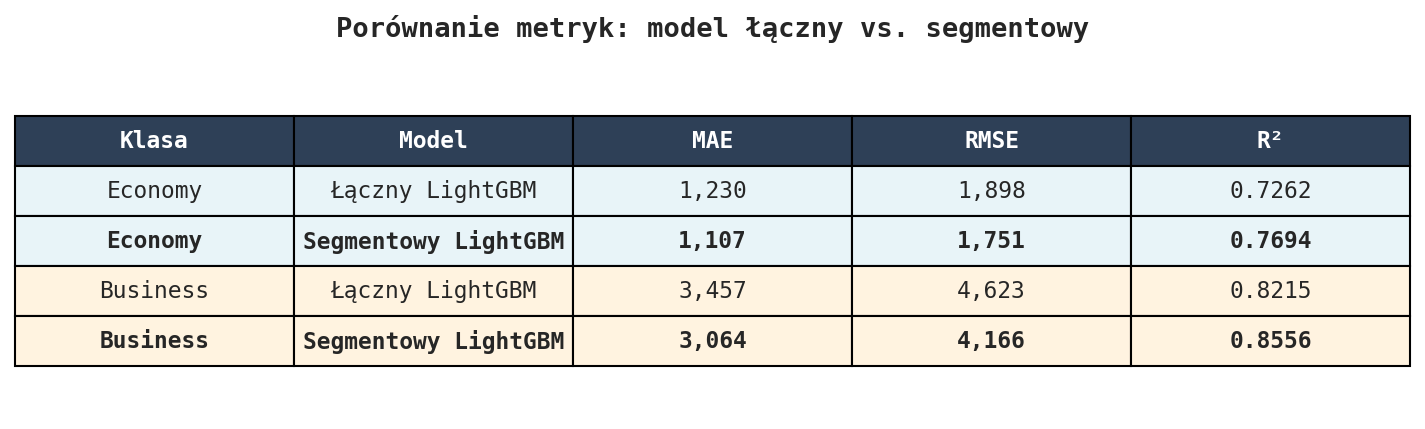
\includegraphics[width=0.93\textwidth]{porownanie_modeli_metryki.png}
		\caption{Porównanie metryk LightGBM: model łączny vs.\ segmentowy.
			Model segmentowy redukuje MAE o~10\% w klasie Economy (z~1\,230 do 1\,107~INR)
			i o~11\% w klasie Business (z~3\,457 do 3\,064~INR). Analogiczne
			polepszenie widoczne jest dla RMSE oraz R², który wzrasta z~0,7262 do
			0,7694 (Economy) i z~0,8215 do 0,8556 (Business).}
	\end{figure}
		Zestawienie metryk modelu łącznego i segmentowego dla algorytmu LightGBM
	jednoznacznie potwierdza przewagę podejścia segmentowego:
	% ══════════════════════════════════════════════════════════════════════════════
	\section{Podsumowanie i Wnioski}
	
	\subsection{Model łączny vs.\ modele segmentowe}
	
	Głównym wnioskiem projektu jest wyraźna przewaga \textbf{podejścia segmentowego}
	nad modelem łącznym. Połączony zbiór Economy + Business tworzy heterogeniczną
	populację, której pojedynczy model nie może optymalnie aproksymować. Osobne
	modele dla każdej klasy:
	
	\begin{itemize}
		\item osiągają wyższe R² i niższe MAE/RMSE w obu segmentach,
		\item lepiej uchwytują specyficzne dla każdej klasy zależności
		(różny wpływ \texttt{days\_left} i linii lotniczej),
		\item eliminują problem ``kompromisowego'' dopasowania.
	\end{itemize}
	
	\subsection{Wybór algorytmu --- LightGBM jako model finalny}
	
	Spośród sześciu testowanych algorytmów \textbf{LightGBM} jednoznacznie wyróżnia
	się jako model finalny z trzech powodów:
	
	\begin{enumerate}
		\item \textbf{Najwyższa dokładność} --- najniższe MAE i RMSE, najwyższe R²
		zarówno w modelu łącznym, jak i w obu modelach segmentowych.
		\item \textbf{Brak przetrenowania} --- w przeciwieństwie do Random Forest,
		który przekracza próg overfittingu w obu klasach (Train R² $-$ Test R² $>$ 0,05).
		\item \textbf{Efektywność} --- czas treningu wielokrotnie krótszy niż
		Random Forest i XGBoost przy porównywalnych lub lepszych wynikach.
	\end{enumerate}
	
	\subsection{Kluczowe predyktory}
	
	Analiza SHAP potwierdza, że \texttt{days\_left} i \texttt{duration} są
	najważniejszymi predyktorami w obu segmentach, choć z różną siłą oddziaływania.
	Silny wpływ zmiennych linii lotniczej wskazuje na znaczące zróżnicowanie cenowe
	między przewoźnikami, nieuchwytne przez modele liniowe.
	
	\subsection{Możliwe kierunki dalszych badań}
	
	\begin{itemize}
		\item Głębszy tuning hiperparametrów z wykorzystaniem Optuna / Bayesian Search,
		\item Integracja zewnętrznych źródeł danych (dni wolne, sezony turystyczne),
		\item Wdrożenie produkcyjne jako API (Flask / FastAPI) z interfejsem webowym.
	\end{itemize}
	
	% ══════════════════════════════════════════════════════════════════════════════
\end{document}